\documentclass[11pt,a4paper]{article}

% Define page geometry
\usepackage{geometry}
\geometry{left=2.2cm,
	right=2.2cm,
	top=2.2cm,
	bottom=2cm}
\parskip 0.15cm
\setlength{\parindent}{0cm}
\usepackage{pdflscape}
\usepackage[document]{ragged2e}

% Set font
\usepackage[T1]{fontenc}

% Image handling
\usepackage{graphics}  % Insert images easily
\usepackage{graphicx}  % Extended image support

\makeatletter
	\g@addto@macro\@floatboxreset\centering  % Automatically centre images (floats)
\makeatother

\graphicspath{ {img/} }
\usepackage{float}  %  Graphics placement [H] [H!] arguments
\usepackage{subfig}  % Compound figures

% Tables
\usepackage{multirow}
\usepackage{longtable}

% Bibliography management
\usepackage[UKenglish]{babel}
\usepackage[natbibapa]{apacite}
\bibliographystyle{apacite}

% Text formatting
\usepackage{url} % Allow nice formatting of URLs in text

\usepackage{enumerate}  % Enumerated lists

\usepackage{lineno}  % Line numbers

\usepackage{textcomp}
\newcommand{\textapprox}{\raisebox{0.5ex}{\texttildelow}}  % Command for a good tilde

\usepackage{siunitx}
\usepackage{amsmath}

\usepackage{xcolor}
\newcommand{\todo}[1]{\textcolor{red}{\textbf{#1}}}   % \todo{NOTE TO SELF WRITTEN IN RED}

\input{code_format}

% Custom title formatting
\let\oldtitle\title

\renewcommand{\title}[1]{\oldtitle{\vspace{-1.5cm}#1}}

\usepackage[breaklinks]{hyperref}
\definecolor{links}{RGB}{191,59,72}
\hypersetup{
	breaklinks,
	colorlinks,
	allcolors=links,
	linktoc=section,
	pdfauthor={John L. Godlee}
}
\def\subsectionautorefname{section}
\def\subsubsectionautorefname{section}
% \usepackage{biblatex}

\usepackage{dcolumn}
\usepackage{multirow}
\usepackage{tikz}
\usetikzlibrary{calc,arrows,positioning,shapes,shapes.gates.logic.US,trees}
\usepackage{pdflscape}
\usepackage{longtable}
\usepackage{fmtcount}

\usepackage{lineno}
\linenumbers

\title{Tree biodiversity and ecosystem function relationship across southern African woodlands}
\author{}
\date{}

\newcommand{\nplots}{1767}
\newcommand{\nplotspcoa}{1877}
\newcommand{\nstems}{93242}

\newcommand{\hullcover}{94.4}

\newcommand{\pcsdsd}{1}
\newcommand{\pcsded}{1.03}
\newcommand{\pcshdh}{1}
\newcommand{\pcshhh}{0.73}
\newcommand{\pcsdb}{-0.14}
\newcommand{\pcshb}{0.41}
\newcommand{\pcsdh}{0.42}
\newcommand{\pcsib}{0.77}
\newcommand{\pcsdi}{0.17}
\newcommand{\strucrsq}{0.7}
\newcommand{\strucbrsq}{0.69}
\newcommand{\struccrsq}{0.72}
\newcommand{\strucsib}{$\beta =$ NA$\pm$NA, p = NA}
\newcommand{\strucbsb}{$\beta =$ -0.25$\pm$0.064, p <0.01}
\newcommand{\strucbhb}{$\beta =$ 0.28$\pm$0.049, p <0.01}
\newcommand{\struccsb}{$\beta =$ 0.14$\pm$0.118, p = 0.24}

\newcommand{\rgmbd}{$\beta =$ 0.02$\pm$0.008, p = 0.06}
\newcommand{\rgsbd}{$\beta =$ 0.02$\pm$0.008, p = 0.05}
\newcommand{\rgid}{$\beta =$ 0.62$\pm$0.034, p <0.01}
\newcommand{\rghb}{$\beta =$ 0.33$\pm$0.042, p <0.01}
\newcommand{\fmrsq}{0.5}
\newcommand{\fmrmsea}{0.166}
\newcommand{\fmtli}{0.905}
\newcommand{\fmcfi}{0.924}
\newcommand{\pcfmmp}{1}
\newcommand{\pcfmmpc}{0.11}
\newcommand{\pcfmmt}{0.17}
\newcommand{\pcfmmtc}{0.57}
\newcommand{\pcfdds}{1}
\newcommand{\pcfdde}{0.72}
\newcommand{\pcfsss}{1}
\newcommand{\pcfsso}{0.31}
\newcommand{\pcfssc}{0.37}
\newcommand{\pcfhhh}{1}
\newcommand{\pcfhhd}{0.96}
\newcommand{\pcfmd}{0.21}
\newcommand{\pcfsd}{0.21}
\newcommand{\pcfdh}{0.3}
\newcommand{\pcfmi}{-0.01}
\newcommand{\pcfsi}{-0.01}
\newcommand{\pcfdi}{0.62}
\newcommand{\pcfsb}{0.03}
\newcommand{\pcfmb}{0.01}
\newcommand{\pcfdb}{0.07}
\newcommand{\pcfhb}{0.33}
\newcommand{\pcfib}{0.49}
\newcommand{\srsq}{46}

\newcommand{\ccib}{$\rho =$ 0.78, p <0.01}
\newcommand{\ccmb}{$\rho =$ 0.24, p <0.01}
\newcommand{\ccmcb}{$\rho =$ -0.09, p <0.01}
\newcommand{\ccob}{$\rho =$ 0.23, p <0.01}
\newcommand{\ccsb}{$\rho =$ -0.25, p <0.01}
\newcommand{\ccms}{$\rho =$ 0.39, p <0.01}
\newcommand{\ccme}{$\rho =$ 0.1, p <0.01}
\newcommand{\ccmh}{$\rho =$ 0.21, p <0.01}
\newcommand{\ccmi}{$\rho =$ 0.12, p <0.01}
\newcommand{\ccsi}{$\rho =$ 0.54, p <0.01}
\newcommand{\ccei}{$\rho =$ 0.47, p <0.01}
\newcommand{\cctb}{$\rho =$ -0.05, p <0.05}
\newcommand{\cctcb}{$\rho =$ -0.19, p <0.01}

\newcommand{\subn}{80}
\newcommand{\subp}{359.4}

\newcommand{\percsmallagb}{2.1}

\newcommand{\nzam}{3760}
\newcommand{\nzamcluster}{940}


\begin{document}

{\LARGE{Title: Tree species and structural diversity are important determinants of ecosystem function across southern African woodlands}}

\vspace{1cm}

Authors: John L. Godlee\textsuperscript{1}, Casey M. Ryan\textsuperscript{1}, David Bauman\textsuperscript{2,3}, Samuel J. Bowers\textsuperscript{1}, Joao M. B. Carreiras\textsuperscript{4}, Antonio Valter Chisingui\textsuperscript{5}, Joris P. G. M. Cromsigt\textsuperscript{6,7,8}, Dave J. Druce\textsuperscript{9,10}, Manfred Finkch\textsuperscript{11}, Francisco Maiato Gon\c{c}alves\textsuperscript{5}, Ricardo M. Holdo\textsuperscript{12}, Steve Makungwa\textsuperscript{13}, Iain M. McNicol\textsuperscript{1}, Edward T. A. Mitchard\textsuperscript{1}, Anderson Muchawona\textsuperscript{14}, Rasmus Revermann\textsuperscript{11,15}, Natasha Sofia Ribeiro\textsuperscript{16}, Abel Siampale\textsuperscript{17}, Stephen Syampungani\textsuperscript{18}, Jos\'{e} Jo\~{a}o Tchamba\textsuperscript{5}, Hemant G. Tripathi\textsuperscript{19}, Johannes Wallenfang\textsuperscript{11}, Mariska te Beest\textsuperscript{20,21,22}, Mathew Williams\textsuperscript{1}, Kyle G. Dexter\textsuperscript{1,23}

1: School of GeoSciences, University of Edinburgh, Edinburgh, EH9 3FF, United Kingdom \\
2: Environmental Change Institute, School of Geography and the Environment, University of Oxford, Oxford, United Kingdom \\
3: Laboratoire d'\'{E}cologie V\'{e}g\'{e}tale et Biogéochimie, CP 244, Universit\'{e} Libre de Bruxelles, Brussels, Belgium \\
4: National Centre for Earth Observation (NCEO), University of Sheffield, Hicks Building, Hounsfield Road, Sheffield, S3 7RH, United Kingdom \\
5: Herbarium of Lubango, ISCED Hu\'{i}la, Sarmento Rodrigues Str. No. 2, CP. 230, Lubango, Angola \\
6: Department of Wildlife, Fish, and Environmental Studies, Swedish University of Agricultural Sciences, Ume\aa, Sweden \\
7: Department of Zoology, Centre for African Conservation Ecology, Nelson Mandela University, Port Elizabeth, South Africa \\
8: Copernicus Institute of Sustainable Development, Utrecht University, 3584CS Utrecht, the Netherlands \\
9: Ecological Advice, Ezemvelo KZN Wildlife, Hluhluwe-iMfolozi Park, South Africa \\
10: School of Life Sciences, University of KwaZulu-Natal, Pietermaritzburg, South Africa \\
11: Biodiversity, Evolution and Ecology of Plants, Institute of Plant Sciences and Microbiology, University of Hamburg, Ohnhorststr. 18, 22609 Hamburg, Germany \\
12: Odum School of Ecology, University of Georgia, 140 E. Green St., Athens, GA 30602, USA \\
13: Lilongwe University of Agriculture and Natural Resources (LUANAR), Lilongwe, Malawi \\
14: Forest Research Center, 1 Orange Groove Highlands, Harare, Zimbabwe \\
15: Faculty of Natural Resources and Spatial Sciences, Namibia University of Science and Technology, Windhoek, Namibia \\
16: Department of Forest Engineering, Faculty of Agronomy and Forest Engineering, UEM Av. Julius Nyerere, 3453, Campus Universitario, Maputo, Mozambique \\
17: Forestry Department Headquarters - MLNR, Cairo Road, Lusaka, Zambia \\
18: School of Natural Resources, Copperbelt University, Kitwe, Zambia \\
19: Faculty of Biological Sciences, University of Leeds, LS2 9JT, United Kingdom\\
20: Copernicus Institute of Sustainable Development, Utrecht University, 3508 TC Utrecht, The Netherlands \\
21: Centre for African Conservation Ecology, Nelson Mandela University, Port Elizabeth, 6031, South Africa \\
22: South African Environmental Observation Network, Grasslands-Forests-Wetlands Node, Montrose, 3201, South Africa \\
23: Royal Botanic Garden Edinburgh, Edinburgh, EH3 5LR, United Kingdom \\

\vspace{1em}
Corresponding author:

John L. Godlee

johngodlee@gmail.com

School of GeoSciences, University of Edinburgh, Edinburgh, EH9 3FF, United Kingdom

\section{Acknowledgements}

This work is funded by a NERC E3 Doctoral Training Partnership PhD studentship at the University of Edinburgh (John L. Godlee, Grant No. NE/L002558/1). The data for this study was contributed by a number of independently funded projects and was assembled and prepared by SEOSAW (A Socio-Ecological Observatory for Southern African Woodlands, \url{https://seosaw.github.io}), an activity of the Miombo Network and a NERC-funded project (Grant No. NE/P008755/1). Revisions of the SEOSAW dataset were funded by SavannaChange, a GCRF/University of Edinburgh funded project. We thank all data providers and the field assistance they received when collecting plot data. JMBC was supported by the Natural Environment Research Council (Agreement PR140015 between NERC and the National Centre for Earth Observation). 

\section{Conflict of interest statement}

All authors declare no conflict of interest regarding this study.

\section{Biosketch}

SEOSAW (A Socio-Ecological Observatory for Southern African Woodlands, \url{https://seosaw.github.io}) aims to understand the response of southern African woodlands to global change. The goal of SEOSAW is to produce novel analyses of the determinants of ecosystem structure and function for the southern Africa region, based on syntheses of plot data. Additionally the group hopes to develop infrastructure for a long-term regional plan for plot remeasurement in the southern African region. While working on a multitude of diverse projects in the dry tropics at large, all authors have a broad interest in community ecology and ecosystem assemblage in southern African woodlands.

\newpage{}

{\LARGE{\textbf{Blinded Main Text File}}}

\LARGE{Title: Tree species and structural diversity are important determinants of ecosystem function across southern African woodlands}

\normalsize{Running title: Diversity - ecosystem function in southern African woodlands}

\section{Abstract}

\textbf{Aim:} Positive correlations between tree species diversity and ecosystem function have been widely documented, but the nature of the relationship in southern African savanna/woodlands, which experience high levels of disturbance through fire and ecophysiological stress, is less clear. It is posited that high levels of disturbance moderate the effects of competition in savannas, weakening the correlation between biodiversity and niche complementarity that drives ecosystem function. Here, we explore the relationship between tree species diversity and aboveground biomass across southern African savannas and woodlands, while controlling for variation in stem density, resource availability, disturbance through fire, and vegetation types to build a general understanding of the biodiversity - ecosystem function relationship in this understudied ecological context.

\textbf{Location:} Southern African savannas and woodlands
\textbf{Time period:} 2010-2019

\textbf{Major taxa studied:} Trees

\textbf{Methods:} We used a network of \nplots{} savanna/woodland tree plots located across the southern African sub-continent. We used Structural Equation Modelling with path analysis to determine the relationship between tree species diversity and aboveground woody biomass, while accounting for the interactive effects of resource availability, disturbance by fire, stem density and vegetation type.

\textbf{Results:} We found a positive effect of tree species diversity on aboveground biomass, across vegetation types, observed mainly via the increasing effect of woodland structural diversity. We also found that the effect of tree species diversity on biomass increases with stem density, with a minimum threshold of \textapprox{}180 stems ha\textsuperscript{-1}. Finally, we found that resource availability affects biomass in southern African woodlands mainly indirectly, via its effect on species diversity, suggesting that tree diversity may have been under-appreciated as a determinant of savanna structure.

\textbf{Main conclusions:} The study underlines the close association between tree diversity and ecosystem structure and function of highly disturbed southern African savannas and woodlands. Our results demonstrate the importance of accounting for environmental conditions and vegetation type in order to accurately model a general relationship between biodiversity and ecosystem function at a regional level. 

\textbf{Keywords:} biodiversity, ecosystem function, woodland, miombo, biomass, structural equation modelling, forest structure.

\section{Introduction}

% BEFR has had previous global research
In order to understand the effects of global biodiversity change, it is necessary to explore the relationship between biodiversity and ecosystem function \citep{Tilman2014}. The strength and direction of the Biodiversity-Ecosystem Function (BEF) relationship varies depending on the ecosystem being studied, the ecosystem function(s) of interest \citep{Hector2007}, and the inclusion of environmental covariates in statistical models \citep{Vila2005}, but there appears to be a generalisable positive correlation between biodiversity and ecosystem function \citep{Liang2016, Hooper2012, Cardinale2009}. Over the past decade, many observational studies of the BEF relationship have been conducted, mostly in wet tropical and temperate forests, and grasslands \citep{Chen2011}, which follow from early small-scale experimental studies conducted predominantly in artificial grassland mesocosms \citep{Tilman1994, Tilman2014}. Despite these concerted efforts, we continue to lack a nuanced, ecosystem-agnostic, understanding of the complex interactions between biodiversity, environment, and ecosystem function.

% Ecosystem function definition and mechanisms
Ecosystem functions can be defined in broad terms as rate processes and aggregate properties of ecosystems that describe the nature of biotic activity within those ecosystems \citep{Jax2005}. This includes processes such as gross primary productivity and atmospheric nitrogen fixation, but can be extended to indirect measures of function such as resilience of productivity to disturbance, and further to ecosystem properties which themselves influence process, such as trophic complexity and total vegetative biomass. The frequently reported BEF relationship invokes three main mechanisms to explain it \citep{Tilman2014}: 1) niche complementarity, whereby communities with greater biodiversity fill a greater breadth of realised niche space and avoid competition due to differences in their resource acquisition strategies; 2) selection effects, whereby communities with greater biodiversity are more likely to include a species that contributes highly to the measured ecosystem function; and 3) facilitation effects, whereby communities with greater biodiversity are more likely to include combinations of species which together increase the others' functional contribution.

% Savannas are big and ecologically important
Savannas and woodlands are the dominant vegetation type across southern Africa, spanning >4 million km\textsuperscript{2} \citep{White1987, Ratnam2011, Ryan2016} (\autoref{clust_map}). The carbon stored in this vegetation is comparable to that found in the wet forests of the Congo basin, and is of global importance to the carbon cycle \citep{Houghton2009, Mayaux2008}. Climatic conditions and biogeography vary across southern African vegetation, resulting in a diverse range of savanna and woodland tree species assemblages. These retain the common features of an open tree canopy and an understorey generally dominated by C4 grasses. Southern African savannas and woodlands are highly diverse, thought to harbour \textapprox{}8500 plant species of which >300 are trees \citep{Frost1996}, and have been identified by previous studies as a priority for conservation efforts \citep{Byers2001, Mittermeier2003}. Many conservation projects in the region currently aim to conserve biodiversity and woody biomass stocks simultaneously under international efforts to reduced deforestation and degradation (REDD+) \citep{Hinsley2015}. Despite these efforts however, human actions are driving rapid changes in biodiversity, with largely unquantified consequences for ecosystem structure and function.

% Savannas might not be the same as forests
Compared to forest ecosystems, southern African dry tropical woodlands and savannas are highly structured by disturbance, through fire \citep{Lehmann2014}, herbivory \citep{Sankaran2008, Levick2009}, and human activities such as shifting cultivation agriculture \citep{Heinimann2017}, timber extraction and charcoal processing \citep{Dewees2010, McNicol2018b}. High levels of disturbance, by fire or otherwise, may weaken the role of competition in determining local species distribution. Disturbance reduces stem density and woody biomass, reducing competitive interactions between individuals, allowing weak competitors to co-exist where they would normally be excluded \citep{Grime1979, Grace1990}. This means that interspecific competition and therefore the effect of niche complementarity, which contributes the majority of the observed biodiversity effect on ecosystem function in temperate and wet tropical forests \citep{Wright2017, Poorter2015, Sande2017a}, may not be as important in dry woodland/savanna ecosystems, thus weakening the BEF relationship. Instead, stress tolerance and the functional contribution of particular species (selection effects) may be the predominant forces influencing ecosystem function \citep{Lasky2014, Tobner2016}. A threshold stem density may exist below which the effects of tree species diversity on ecosystem function are not detectable, with potential consequences for our classification of ecosystems limited by biodiversity and those limited by other factors.

% Savannas might no be the same as forests continued: facilitation effects
More diverse species assemblages may lead to facilitation effects between certain species combinations under the limiting environmental conditions prevalent across African savannas, such as low water availability. Across European forests \citet{Ratcliffe2017} found stronger positive relationships between tree species richness and various ecosystem functions in more arid environments. They suggest that in water-limited ecosystems, facilitative effects and selection effects may be more important than niche complementarity in driving the relationship between species diversity and ecosystem function, as competition diminishes in ecosystems where environmental stress limits individual species' abundances, thus reducing the competition which drives niche complementarity effects. This potential mismatch in the contribution of different mechanisms to the BEF relationship between dry tropical woodlands and other forested ecosystems demands further investigation if we are to derive a generalisable BEF relationship.

% African savannas are understudied in this regard
The representation of dry tropical ecosystems in the BEF relationship literature is poor compared to other ecosystems. \citet{Clarke2017} conducted a meta-analysis of 182 published BEF relationship studies, finding that only 13\% were conducted in the tropics generally, with 42\% of those being conducted in the wet tropical forests of Costa Rica, a narrow geographic region \citep{Barthlott2005}. A severe lack of study in dry tropical ecosystems, especially given the potential divergence in BEF relationship mechanisms described above, suggests that a focus on the BEF in southern African woodlands could greatly strengthen our understanding of a global BEF relationship and its environmental determinants. A small number of studies in southern African woodlands, all of which were restricted in spatial scope to a small region of miombo woodland, found that above-ground woody carbon/biomass stocks correlate positively with tree species richness \citep{McNicol2018, Shirima2015, Mutowo2012}. The results of these fine-scale studies concur with similar studies in other biomes \citep{Cardinale2009}. Studies of the BEF relationship often find that at fine spatial scales (<1 ha), biodiversity shows a strong effect on ecosystem function, but at broad spatial scales  (>10000s ha) biodiversity effects pale in significance compared to abiotic factors such as climate \citep{Pasari2013}. 

% \citep{Michaletz2014, Michaletz2018} \citep{Spasojevic2014}
%In wet tropical forests in Central America, \citet{Condit2013} found that dry season intensity was the main determinant of tree species distribution and abundance evenness.
% Due the potential importance of environment and biogeography in defining the strength and form of a relationship between biodiversity and above ground woody biomass, it is important to sample across broad geographic and environmental gradients to gain understanding of the spatial variation in the relationship between biodiversity and biomass. 
% Environment affects the BEF relationship, so must be accounted for.
Environmental heterogeneity is known to affect both woody biomass and tree species diversity independently, in a number of different biomes \citep{Spasojevic2014, Michaletz2018, Michaletz2014}. Southern African woodlands particularly, occur over a wide range of precipitation, diurnal and annual temperature, and disturbance regimes \citep{Frost1996}. It is important therefore to account for this environmental heterogeneity and understand how it influences both biomass and biodiversity to effectively model and correctly attribute the effects of biodiversity on woody biomass. \citet{Sankaran2005} and \citet{Lehmann2014} both report independently that total precipitation sets the upper limit for woody biomass in African savannas. \citet{Lehmann2014} also report complex indirect relationships between climate, disturbance by fire and woody biomass, demonstrating the need for directional multi-facetted modelling techniques to properly account for the effects of climate. 

% Disturbance deserves another look
High levels of disturbance in southern African woodlands may moderate the observable BEF relationship through its effect on ecosystem composition. Fire disturbance in forests has been linked to abundance-dependent mortality among smaller trees \citep{Roques2001, Staver2009, Bond2005}. Some species in the regional species pool may be excluded from woodland plots with high levels of disturbance if they are unable to escape the fire bottleneck and grow to become a large tree. Selection effects may therefore be more important in maximising ecosystem function in disturbance-prone woodlands. If a given woodland plant community contains a large number of species, it is more likely that one of them will possess the necessary growth strategy to grow to a large tree with high biomass under an intense disturbance regime. 

% Structural diversity is important too
Southern African woodlands possess structurally diverse tree canopies, with trees occupying distinct layers of the canopy, depending on their growth stages and species identity \citep{Solbrig1996}. This structural diversity may be one mechanism through which tree species diversity influences woody biomass. \citet{Kunz2019} found that crown complementarity and crown plasticity both increased with species richness in a seasonally dry subtropical forest. They also found that trees growing in species-rich neighbourhoods exhibited enhanced biomass production. Occupancy of multiple canopy layers allows a fuller canopy with  greater total foliage density, enhancing productivity and allowing greater standing woody biomass in a smaller area via a form of niche complementarity. This mechanism however, which has been supported by experiments and observational studies in temperate and wet tropical ecosystems \citep{Hardiman2011, Stark2012}, may not be relevant in savannas. Instead, the overriding importance of disturbance history may negate the effects of tree species diversity on structural diversity \citep{Grime2012}.

% In this study :::
In this study, we made the first known regional estimation of the biodiversity-ecosystem function relationship across southern African savannas and woodlands, using inventory plots spanning broad environmental and biogeographical gradients (\autoref{clust_map}). We used aboveground woody biomass of trees as our metric of ecosystem function, and compared the relative effects of tree species diversity with that of environmental factors known to affect ecosystem productivity and biomass accumulation, namely water availability and soil fertility. We also investigated the potential moderating effects of environmental covariates on the relationship between tree species diversity and biomass. We incorporated vegetation type (via clustering of plot-level tree species composition), as a factor in our analyses to understand how tree species composition as well as diversity affected ecosystem function and to assess the generality of our results. We used Structural Equation Modelling (SEM) with path analysis to simultaneously account for environmental and biotic factors, which may have interacting effects on ecosystem structure and therefore biomass. Initially, we posited three hypotheses: (1) water availability and soil fertility will indirectly positively affect woody biomass via an increase in tree species diversity, (2) the effect of tree species diversity on woody biomass will increase with plot-level stem density (number of stems ha\textsuperscript{-1}), due to an increased importance of niche complementarity as stem density and therefore competition increases. In addition, we expect that an increase in disturbance by fire will decrease stem density and therefore competition, weakening the effect of tree species diversity on woody biomass. Finally, we expect that (3) tree species diversity will increase tree structural diversity (i.e. physiognomic diversity), providing an indirect path by which tree diversity increases woody biomass.

\section{Materials and methods}

\subsection{Study location}

% Situation
The study used \nplots{} woodland monitoring plots from the larger SEOSAW network \citep{seosaw_web} located across 10 countries within southern Africa in the miombo ecoregion (\autoref{clust_map}; \citealp{White1987}). The study area spans the core climate space of the region, with a precipitation gradient from \textapprox{}460 mm y\textsuperscript{-1} in southern Mozambique and southern Zimbabwe to \textapprox{}1700 mm y\textsuperscript{-1} in northern Zambia, Malawi and northern Mozambique. A 2D convex hull of Mean Annual Precipitation (MAP) and Mean Annual Temperature (MAT) of the study sites covers \hullcover{}\% of the pixel-wise climate space of the miombo woodland ecoregion \citep{White1987}, using WorldClim estimates of Mean Annual Temperature (MAT, BIO1) and Mean Annual Precipitation (MAP, BIO12) between 1970 and 2000 with a pixel size of 30 arc seconds (926 m at equator) \citep{Fick2017}. 

% Plots chosen
Plots were chosen from a larger pool of 5395 plots held in the SEOSAW database \citep{seosaw_web} based on the quality and completeness of data collection, and plot setup. Plot vegetation was identified under the broad term of ``savanna'', which includes ``woodland'', ``savanna woodland'', and ``tree savanna'', variously defined in other areas of the scientific literature and here referred to collectively as southern African woodlands \citep{Ratnam2011, Hill2010}. Plots with evidence of farming, human resource extraction or experimental treatments such as prescribed burning or herbivore exclusion were excluded from the initial pool. Only plots >0.1 hectares were used in analyses, as area-based biomass estimation from small plots is highly influenced by rare large trees \citep{Stegen2011}, leading to inaccurate estimates. Only plots with a stem density >50 trees ha\textsuperscript{-1} (>10 cm stem diameter) were used, to ensure all plots represented woodland rather than ``grassy savanna'', which is considered a separate biome with very different species composition \citep{Parr2014}. 

% Zambia disclaimer
\nzam{} plots provided by the 2005-2008 Zambian Integrated Land Use Assessment \citep{Mukosha2009, Pelletier2018} were arranged in clusters of four 20x50 m plots, 20 metres apart. Data from each plot within a cluster were combined and treated as a single plot in analyses, resulting in \nzamcluster{} aggregate plots which were then subject to the plot filtering process described above.

\subsection{Data collection}
 
% AGB
We considered only trees and shrubs in our calculations of Above-Ground woody Biomass (AGB), including woody species such as palms and cycads, which are functionally tree-like. Woody lianas are scarce in our study plots and were not measured. Only stems >10 cm DBH (Diameter at Breast Height, 1.3 m) were included in analyses. Many plots in the dataset did not include data on stems <10 cm DBH. For those plots which contained stem measurements <10 cm DBH, small stems only accounted for a median of \percsmallagb{}\% of the plot level AGB. 

% Number of stems
All stems >10 cm DBH were measured within each plot resulting in a total of \num[group-separator={,}]{\ntrees{}} stems with measurements. A tree may be comprised of multiple stems and so tree-level richness estimates, rather than stem-level estimates, were used to prevent bias from species which readily coppice. For each tree, we recorded species, DBH and tree height to the top of the highest branch material. Height was measured through a variety of means including laser rangefinders, manual clinometers and measuring sticks. When DBH could not be measured at 1.3 m due to trunk abnormalities, it was measured at the closest regular portion of the trunk to 1.3 m. The height of this measurement was recorded and used to estimate the DBH\textsubscript{e} at 1.3 m using a cubic polynomial regression, with parameters estimated using a test dataset from Ryan C., (unpublished), see \citet{Godlee2020}.

% AGB Calculation
AGB for each plot (t ha\textsuperscript{-1}) was calculated using \autoref{chave_agb}, taken from \citet{Chave2014}:

\begin{equation}
	AGB = 0.0673 \times (\rho D^{2} H)^{0.976}
	\label{chave_agb}
\end{equation}

where $\rho$ is the species mean wood density (g cm\textsuperscript{-3}), $D$ is the DBH\textsubscript{e} (cm) at 1.3 m, and $H$ is the tree height (m). Wood density estimates were taken from the global wood density database for each species where possible \citep{Chave2009, Zanne2009}. Wood density for species without species level estimates was estimated from the means of their respective genera. For stems where tree height was unknown, the plots' climatic parameters, estimated from plot location, were used to estimate tree height, according to \citet{Chave2014}.

% WorldClim, SoilGrids and MODIS
Climatic data were taken from the WorldClim database, using the BioClim variables \citep{Fick2017}. In addition to MAT and MAP, temperature stress was calculated as the mean diurnal temperature range (BIO2) and precipitation seasonality was calculated as the mean of the coefficient of variation of monthly mean precipitation (BIO15). Soil fertility data were extracted from the ISRIC gridded soil information data product at 250 m resolution, taking the grid cell value for each plot centre \citep{Hengl2017}. We extracted Cation Exchange Capacity (CEC) (cmolc kg\textsuperscript{-1}), soil organic carbon stocks (kg m\textsuperscript{-2}) percentage soil sand content (0.05-2 mm) by weight and soil nitrogen content (g kg\textsuperscript{-1}). These data are a modelled product derived from various remotely sensed and directly measured data sources. The degree of fire disturbance was calculated using the MODIS monthly burned area product at 500 m resolution (MCD64A1; \citealt{MODIS_burn}), counting the total number of times the plot pixel was classified as burning, between 2001 and 2018. We initially aimed to include disturbance by herbivory in our model, including total herbivore biomass from the \citet{Hempson2017} modelled herbivory product, but this inclusion prevented models from converging due to its collinearity with other observed variables, notably MAP and disturbance by fire. 

\subsection{Data analysis}

\subsubsection{Species diversity and structural diversity metrics}

Estimated tree species richness was calculated for each plot using `ChaoRichness()' from the `iNEXT' package in R \citep{Hsieh2016}. This procedure extrapolates a species rarefaction curve to its predicted asymptote and uses this value as its estimated species richness value. Extrapolated species richness accounts for variation in plot size (0.1-10 ha) and therefore sampling effort among plots. Larger plots will tend to encompass more individuals, and therefore more species \citep{Dengler2009}. To measure tree species evenness, the Shannon Equitability index ($E_{H'}$) \citep{Smith1996} was calculated as the ratio of the estimated Shannon diversity index to the natural log of estimated species richness. Abundance evenness allows for greater niche complementarity at small scales due to potentially increased heterogeneity of functional traits. We quantified tree structural diversity for each plot by calculating the coefficient of variation of DBH (DBH CoV) and tree height (Height CoV). 

\subsubsection{Vegetation clusters}

Plots were assigned to vegetation type groups based on tree species composition. Groups were defined in a manner adapted from \citet{Fayolle2018} in an Africa-wide analysis of floristic units using plot data in savannas and woodlands with tree species diversity and relative abundance data. Group identification was conducted using unconstrained correspondence analysis, followed by hierarchical clustering based on dominant ordination axes. Plot data used in this study occurred in four compositional vegetation types. See \autoref{clust_summ} for a description of each vegetation cluster and \autoref{clust_map} for the spatial distribution of plots from each of these clusters. Cluster names were assigned post-hoc based on the dominant and indicator species in each cluster.


\subsubsection{Structural Equation Modelling}

We used Structural Equation Modelling (SEM) to investigate the determinants of AGB. All SEMs were constructed and analysed in the `lavaan' package \citep{lavaan} in R version 3.6.0 \citep{R2019}. SEM was used because of its suitability for modelling complex causal interactions in ecological systems \citep{Lee2007}. A key aspect to our decision to use SEM is that they can explicitly model and partition variance attributed to indirect effects, which is challenging in standard multiple regressions. Using SEMs also allowed us to describe latent variables such as ``water availability'', ``soil fertility'', and ``disturbance'' which have been suggested to act upon biodiversity and biomass/productivity in previous studies despite these factors not having directly observable measures in our dataset. SEM is also necessary to properly account for potential feedback mechanisms between aspects of environment and tree species diversity, which could otherwise increase the chances of Type I error and wrongly attribute inference due to the covariance of explanatory variables when using conventional regression analyses \citep{Nachtigall2003}.

Prior to analysis, we specified a conceptual model with factors expected to affect AGB: water availability, soil fertility, disturbance, tree species diversity, tree structural diversity and stem density (\autoref{con_mod}). 

Observed variables were transformed to achieve normality where necessary and standardised to Z-scores prior to analysis (\hyperref[appendixa]{Appendix A}). Standardisation allows path regression coefficients to be easily compared between paths in the same model to assess their relative effect size, and eliminates confusion in model interpretation arising from the observed variables being on different scales \citep{Beaujean2014}. Standardisation also controls for variables with variation across different orders of magnitude, which could otherwise prevent adequate model estimation from the covariance matrix in `lavaan'. To ensure that observed variables within a latent variable had consistent directions of influence, some observed variables had their sign reversed. For example, overall water availability is expected to decrease as soil sand content increases, therefore sand content was reversed for use in the water availability latent variable. Precipitation seasonality, and temperature stress were also reversed in this way to account for the direction of their effect on water availability. 

The factor loadings of the observed variable assumed to contribute most to each latent variable were set to one, as per convention, with other observed variables being allowed to vary \citep{Beaujean2014}.  We tested the robustness of our assumptions with a chi-squared test of all possible combinations of observed variable factor loadings set to one, while ensuring no factor loadings were in excess of one. We found no significant difference between model specifications (p>0.05). Full Information Maximum Likelihood (FIML) was used in each model to estimate the values of missing data in each latent variable \citep{Cham2017}.

We assessed the role of tree species diversity and tree structural diversity in determining AGB via a simple mediation model which allowed species diversity to influence AGB both directly and indirectly via structural diversity. Structural diversity can also directly influence AGB in this model, separate to the effect of of species diversity. To account for variation in stem density, which may covary with species diversity, we included it as an observed variable in our model. To explore variation in the model among woodland vegetation types, we fit the model both at the regional scale and for each vegetation type separately. We compared unstandardised path coefficients among the models for different vegetation types to understand the effect that vegetation type has on the relationship between tree species diversity, structural diversity, stem density and AGB. Path coefficients show the effect of a given path with other paths held constant. Models were estimated using the ``MLM'' estimator, because it is robust to multivariate non-normality \citep{Shapiro1983}. Model fit was evaluated using the robust Comparative Fit Index (CFI), the robust Tucker Lewis Index (TLI), the Root Mean Squared Error of Approximation (RMSEA) and the R\textsuperscript{2} coefficient of determination for AGB. We critically assessed model fit in each case, taking into consideration the recommendations of \citet{Hu1999} who define threshold values of acceptability for these model fit indices: CFI >0.85, TLI >0.85, RMSEA <0.15, alongside our judgement of the model estimates.

To explore the hypothesis that niche complementarity effects increase in strength as stem density increases, we repeatedly sub-sampled the available plot dataset to create \subn{} datasets of similar size with varying median stem density. We used each of these datasets separately to fit the model including only tree species and structural diversity latent variables to predict AGB. We excluded the effect of stem density on AGB and the correlation between stem density and species diversity from this model as we deliberately controlled stem density in our subsampling. We then examined how the unstandardised path coefficients for each path in the SEM varied according to the median stem density of subsampled datasets. Preliminary analyses that included herbivore biomass \citep{Hempson2017} did not converge, possibly due to the spatially coarse nature of the available data, we therefore did not include herbivory in our final model. We incorporated environmental covariates into our model to understand the relative effects of water availability, soil fertility and disturbance on AGB both directly and indirectly via species diversity and stem density. We compared standardised path coefficients between paths in the model to understand the relative contribution of each path to explain variance in AGB. Vegetation type specific models could not be reliably fitted for this more complex model specification with environmental covariates, due to sample size issues and because some vegetation types were narrow in their climate space, leading to a lack of environmental variation, particularly in the water availability latent variable.

\section{Results}


% Correlations
Pairwise correlations between all observed variables used in the Structural Equation Models (SEMs) showed that all tree species diversity and structural diversity variables had moderate positive correlations with AGB. Stem density had the strongest correlation with AGB of all variables considered (\ccib{}). Environmental variables had weaker correlations with AGB than diversity variables, with all environmental variables having significant correlations with AGB, except fire frequency. The direction of these correlations was used as a test of our assumptions for the direction of influence of latent variables later used in the SEMs. MAP had positive correlations with all tree species diversity and structural diversity variables. Tree species diversity variables had clear positive correlations with stem density (species richness: \ccsi{}; Shannon equitability: \ccei{}), but structural diversity variables showed weak correlations with stem density (DBH CoV: \ccdvi{}, Height CoV: \cchvi{}).

\subsection{Structural and species diversity models}

In an SEM describing the effect of tree species diversity on AGB via the mediating effects of tree structural diversity and stem density (\autoref{struc_mod}), species diversity showed no direct effect on AGB (\strucbetadb{}), but did have an indirect positive effect via structural diversity (\strucbetadib{}) (\autoref{struc_mod}). Model fit was good with high factor loadings for all observed variables. All other path coefficients were significant (p <0.01) (\autoref{struc_model_fit_clust_stats}). The R\textsuperscript{2} of AGB was \strucrsq{}. The strongest direct effect on AGB was from stem density (\strucbetaib{}).


\subsection{Variation among vegetation types}

When the tree species and structural diversity model (\autoref{struc_mod}) was refitted separately using data from each of the four vegetation types, we found that the effect sizes of each latent variable remained largely similar, though model fit varied. The direct effect of tree species diversity on AGB was positive and marginally significant in ex-Acacia (\strucbetacsb{}) but negligible in Mopane (\strucbetadsb{}), sparse miombo / \textit{Baikiaea} (\strucbetaasb{}) and Core miombo (\strucbetabsb{}) (\autoref{struc_model_slopes_all}). Relationships between structural diversity and AGB remained generally similar, with the same sign and overlap between the 95\% confidence intervals of path coefficients. The R\textsuperscript{2} of AGB was highest in ex-Acacia shrubland (R\textsuperscript{2} = \struccrsq{}) and lowest in sparse miombo / Baikiaea (R\textsuperscript{2} = \strucarsq{}). The total effect of species diversity on AGB remained strongly positive for all vegetation types. All vegetation types exhibited a positive effect of species diversity on structural diversity. All models had adequate goodness-of-fit (\autoref{struc_model_fit_clust_stats}), though confidence intervals around the unstandardised path coefficients were wide particularly for Mopane and ex-Acacia. $\chi^{2}$ statistics were high for some vegetation types, but this appears to be highly correlated with sample size for each vegetation type \citep{Hooper2008}.


\subsection{Moderation of Diversity-AGB relationship by stem density}

In our sub-sampling of the plot dataset by stem density, we found an increasing positive effect of tree species diversity on AGB as stem density increased (\autoref{sem_struc_stems_ha}). There appears to be a minimum stem density threshold at \textapprox{}180 trees ha\textsuperscript{-1} below which there appears to be a reasonably constant baseline effect of tree diversity on biomass. The effect of structural diversity on AGB appears to remain constant with increasing stem density. The indirect effect of tree species diversity on AGB via structural diversity climbs as stem density increases. 


\subsection{Environmental covariates and tree diversity}

A model incorporating the latent variables of water availability, soil fertility and disturbance by fire showed that the total effect of tree species diversity on biomass was similar to that of water availability, soil fertility and disturbance (\autoref{full_mod}, \hyperref[appendixd]{Appendix D}). The direct effects of water availability, soil fertility and disturbance on AGB were negligible (water: \fmbetamb{}, soil: \fmbetasb{}, disturbance: \fmbetafb{}), with nearly all of their observed effect on AGB coming from the indirect paths via stem density (water: \fmbetamib{}, soil: \fmbetasib{}, disturbance: \fmbetafib{}) and species diversity (water: \fmbetamd{}, soil: \fmbetasd{}, disturbance: \fmbetafd{}). MAP and soil sand content had the greatest contributions to the latent variable of water availability. Model fit was acceptable: CFI = 0.925, TLI = 0.900, and RMSEA = \fmrmsea{}, R\textsuperscript{2} of AGB = \fmrsq{}. 

Similar to the model that only considered tree species and structural diversity (\autoref{struc_mod}), the direct effect of species diversity on structural diversity was positive, while structural diversity itself had a positive effect on AGB, leading to a strong positive indirect effect of species diversity on AGB via structural diversity (\fmbetadhb{}) when environmental covariates were accounted for. Again, the direct effect of species diversity on AGB was negligible (\fmbetadb{}). The total effect of species diversity on AGB was positive (\fmbetatotaldb{}). Compared to the simple model with no environmental covariates, the total explanatory power of tree species diversity and structural diversity in this model decreased, but the predictive power of the model as a whole increased.


\section{Discussion}

% Re-cap
In this study, we assessed the importance of [a] tree species diversity, [b] tree structural diversity, [c] resource availability, [d] disturbance by fire, [e] stem density and their interactions on above-ground woody biomass (AGB) across southern African woodlands, using a network of \nplots{} woodland plots. Using Structural Equation Modelling (SEM), we found support for a general positive relationship between tree species diversity and AGB, operating indirectly via structural diversity (H\textsubscript{1}). Tree species diversity, structural diversity and stem density accounted for \smrsq{}\% of the variation in AGB across the region, while models for specific vegetation types showed even greater explanatory power in some cases (\autoref{struc_model_fit_clust_stats}). We found that the effect of tree species diversity on AGB increased with stem density (H\textsubscript{2}), with an apparent threshold of 180 stems ha\textsuperscript{-1} below which the effect of species diversity on AGB remained at a low baseline level. The strongest effect on AGB was that of stem density. When the effects of water availability, soil fertility and disturbance by fire were controlled for, the total explanatory power of tree species diversity and structural diversity decreased, but the predictive power of the model increased, suggesting that it is important to control for environmental covariates to understand the true effect of tree species diversity on AGB in regional scale assessments in southern African woodlands.

\subsection{Inter-related effects of tree species and structural diversity on AGB}

% 
We found a consistent positive effect of tree species diversity on AGB across all models in the current study. Within southern African woodlands we therefore find support that higher tree species richness and evenness leads to higher woody AGB. This finding is in agreement with many other studies across different ecosystems and biomes, supporting the idea that there is a generalisable positive association between biodiversity and ecosystem function \citep{Liang2016, Cardinale2009}. Our study provides a novel dissection of the mechanisms underlying this relationship, particularly in the context of southern African woodlands, a disturbance-structured and poorly studied ecological system.

Much of the total variation in AGB was driven by variation in stem density. It is possible that within southern African woodlands a higher species diversity allows for a higher stem density through niche separation, which reduces competition between species occupying varying niche space, leading to an increase in total AGB per unit area. The opposite causation is also plausible however, with increased stem density causing higher species richness through an increased probability of encountering new species. We attempted to correct for the correlation between species richness and stem density using extrapolated species richness, which extrapolates a rarefaction curve to its predicted asymptote, thus estimating the total landscape-level species richness which is unaffected by plot size and stem density. We suggest therefore that an increase in tree species diversity through species richness and evenness produces an assemblage of species which can utilise more available light and moisture, resulting in greater plot-level AGB. This is supported by the moderately strong indirect positive effect of tree species diversity on AGB via structural diversity, and the positive effect of water availability on AGB via stem density in the model which included environmental covariates. 

We found evidence that tree species diversity led to an increase in AGB indirectly via tree structural diversity, and we therefore find support for our second hypothesis H\textsubscript{2}. A higher tree species diversity allows for a greater structural diversity of trees, i.e. greater variation in DBH and height. This may act as a mechanism for niche complementarity, with a canopy of diversely sized trees able to take advantage of a greater proportion of the available light. Although we did not measure them here, we would also expect that tree species diversity allows for a greater range of tree functional forms \citep{Pretzsch2014}, i.e. wider variation in canopy shape and overall growth form; broad flat crowns vs. narrow deep crowns, for example. In forests, where the tree canopy is effectively closed, as the stand matures a more diverse canopy emerges via competition and tree mortality events which open canopy gaps \citep{Muscolo2014}. Indeed, our finding that the strength of the effect of tree diversity on AGB increases with stem density supports this mechanism. In frequently disturbed woodlands such as those studied here however, a woodland canopy similar to that of a forest is frequently not reached. Instead, a simple open canopy is maintained that can be made more complex and productive via an increase in species diversity. Previous studies have found that southern African woodlands with higher species diversity tend to experience less frequent disturbance by fire and tend to form a more closed canopy and a more sparse understorey \citep{Chidumayo2013, Mutowo2012}. In our study however, we found a positive effect of disturbance on species diversity, perhaps suggesting that disturbance prevents domination of woodlands by a single dominant species \citep{Chidumayo2013}.

We found a non-linear positive effect of stem density on the relationship between tree species diversity and AGB (\autoref{sem_struc_stems_ha}). At low stem densities, competition between mature trees may not occur, meaning that the niche complementarity effect provided by an increase in tree species richness may not be present, accounting for the small effect of tree species diversity on AGB below \textapprox{}180 trees ha\textsuperscript{-1}. At very high stem density, there is also an increase in the effect of species diversity on structural diversity. This could be because at high stem density, the adaptation of different species to growth form become important. At low stem density, individual trees tend to spread out rather than growing tall, but at high stem density, only certain species are able to exist in the understorey, while others are able to grow tall above the woodland canopy, leading to greater variation in tree height over the plot.

\subsection{Effects of water availability, soil fertility and disturbance}

Water availability had a positive total effect on AGB, comparable in size to the total effect of tree species diversity on AGB, while soil fertility had a negative total effect. We expected that higher water availability and soil fertility would lead to higher AGB under the assumption that higher resource availability would allow for a greater stem density per unit area, greater productivity per unit area and additionally greater tree species diversity due to niche partitioning \citep{Kraaij2006, Shirima2015}. Previous studies in tropical forests have shown that water availability increases AGB both directly and indirectly via increasing tree species diversity and via increasing stand structural diversity \citep{Ali2019a, Ali2019b, Poorter2017}. In this study, we observed indirect positive effects of water availability on AGB via species diversity and a positive but only marginally significant direct effect on AGB. Compared to moist tropical forests, water availability is more of a limiting factor to tree growth in southern African woodlands, which experience frequent drought. Disturbance by fire had a negative total effect on AGB. We found negligible indirect effects of disturbance on AGB via species diversity and structural diversity. 

A negative total effect of soil fertility on AGB is in contrast to other studies in the region and against general ecological theory, which predicts a positive effect of soil nutrients on biomass. The negative total effect of soil fertility on AGB was driven mostly by an indirect negative effect via stem density. The direct effect on AGB however, remained positive and marginally significant, as expected. Model estimates of the effect of soil on AGB were poorly constrained compared with other latent variables. This wide standard error on the model predictions is possibly due to the coarseness and nature of the soil data we used. SoilGrids provides modelled data at 250 m resolution, while soil structure and nutrient content varies at much finer scales \citep{Muledi2017, Bucini2007} in southern African woodlands, often being further structured by the vegetation overlying it, an aspect which SoilGrids does not model precisely. Due to the plots used in this study often being situated non-randomly in the landscape, coupled with the coarseness of the SoilGrids data, it is not surprising that this model path is poorly constrained. Soil data is time-consuming to collect and difficult to compare across studies when different protocols are used, though this study prompts the need for further effort in this regard, which may reveal interesting findings about the complex interactions between soil, disturbance and tree diversity in southern African woodlands. \citet{Lehmann2014} similarly found weak and poorly constrained relationships for soil in a Structural Equation Model including precipitation, temperature, soil, fire and tree basal area.

\subsection{Vegetation type responses}

All four vegetation types produced similar results in the simple SEM, with a positive total effect of species diversity on AGB, the majority being indirectly via structural diversity. This demonstrates the robustness of our results, showing they are generalisable across vegetation types in southern Africa. It also demonstrates that similar ecosystem processes are occurring in these vegetation types, despite variation in species composition, overall species richness and mean biomass.

Core miombo and sparse miombo / Baikiaea woodland vegetation exhibited a small negative direct effect of tree species diversity on AGB, while the total effect, incorporating the indirect effect via structural diversity, remained positive in these vegetation types. Compared to ex-Acacia and Mopane woodlands, miombo woodlands have higher median tree species richness. Ex-Acacia and Mopane woodlands are dominated by fewer tree species, notably \textit{Senegalia} spp. in ex-Acacia woodlands and \textit{Colophospermum mopane} in Mopane woodlands which often produce large canopy dominating trees. We postulate that the slight negative effect of tree species richness on AGB in miombo woodlands may be due to an increase in interspecific competition through canopy crowding, but that this effect is not present in ex-Acacia and Mopane woodlands, where the top level of the woodland canopy is dominated often by a single species. 

Higher functional redundancy among tree species in miombo woodlands may lead to smaller trees with lower AGB in the most diverse plots, more resembling thicket vegetation and suppressing the few species which tend to create high biomass, such as \textit{Julbernadia} and \textit{Brachystegia} spp.. In the species-poor Mopane and ex-Acacia woodlands however, the addition of extra species may fill a greater proportional niche space, thus increasing total AGB more. 

Despite Mopane woodland having very low species diversity generally, with often monospecific stands \citep{Timberlake2010}, a positive effect of tree species diversity on AGB was observed. In previous studies across ecosystem types it has been found often that the effect on ecosystem function of adding species is stronger in low diversity assemblages \citep{Hector2007}. This has been attributed to an increase in functional redundancy as species diversity increases. In other words, with more species, it is more likely that the addition of a new species will occupy the same ecological niche space as an existing species, meaning niche complementarity will not occur and competition will not lead to niche partitioning, making little difference to overall ecosystem functioning. Mopane woodlands also have a negligible effect of species diversity on structural diversity. This may be due to the species which tend to co-exist with \textit{C. mopane}, many of which are small shrub-like trees and which do not grow into large canopy trees \citep{Timberlake2010}. Larger canopy trees tend to have greater variation in physical structure \citep{Seidel2019}. 

Ex-Acacia woodlands showed the strongest total effect of species diversity on AGB and was the only vegetation type to show a significant positive direct effect of species diversity on AGB. Ex-Acacia woodlands also had relatively low median species richness compared to miombo, but the addition of new species appears to make a larger difference to the AGB of these plots than in Mopane woodlands. We suggest that this is due mostly to the particular identity of species found in ex-Acacia woodlands and their contribution to ecosystem functioning. Unlike Mopane woodlands, ex-Acacia woodlands contain a wider variety of species which can grow to large canopy trees, albeit at low densities, especially in transition zones with miombo woodlands. 

\subsection{Conclusion}

In this study we found that even in highly disturbed southern African woodlands, there exists a generalisable positive association between tree species diversity and ecosystem function, quantified as above-ground woody biomass (AGB). Additionally, we found that much of the effect of species diversity on biomass exists as an indirect effect by increasing the structural diversity of trees. We found that the multiple vegetation types which comprise southern African woodlands exhibit similarities in the relationship between species diversity and woody biomass, suggesting that similar ecosystem processes occur across the region to determine ecosystem function. In contrast to previous studies, we found, at the scale of our study region, that the direct effects of water availability and soil fertility on woody biomass were small, with most of their effect being indirectly through their effects on tree species and structural diversity. This strongly suggests that data on tree species diversity be included into models predicting ecosystem functionality in this region. We also advocate for explicit inclusion of environmental covariates in regional scale models of biodiversity and ecosystem function, generally. 

The presence of a stem density threshold above which the effect of tree species diversity on AGB increases clearly implies the presence of niche complementarity effects in southern African woodlands, an aspect which has often been overlooked in favour of disturbance effects. On a practical note, our study shows that biodiversity change through human actions will have the greatest negative impact on ecosystem function in areas of high stem density, and low species diversity, which are those areas predominantly targeted for tree felling. This raises concerns about the robustness of these ecosystems to further resource extraction and biodiversity loss. 

\bibliography{regional_befr_manuscript.bib}

\newpage{}

\section{Author contribution statement}

JG and KD conceived the study. JG conducted data analysis, data management for further versions of the SEOSAW dataset, and wrote the manuscript. CR conceived the SEOSAW database and conducted data management for earlier versions of the SEOSAW dataset. JG, CR, DB, JMBC, MF, RH, EM, SS, HT, HT, MB, MW, and KD contributed to manuscript revisions. JG, CR, SB, VC, JPGMC, DD, MF, FG, SM, IM, AM, RR, NR, AS, SS, JT, JW, MB, and MW contributed to experimental design, field data collection, data preparation and data management of parts of the dataset used in this study. 


\begin{landscape}
\section{Tables}

% Table created by stargazer v.5.2.2 by Marek Hlavac, Harvard University. E-mail: hlavac at fas.harvard.edu
% Date and time: Thu, Dec 12, 2019 - 12:06:51
\begin{table}[!htbp] \centering 
  \caption{} 
  \label{clust_summ} 
\begin{tabular}{@{\extracolsep{5pt}} ccccccc} 
\\[-1.8ex]\hline 
\hline \\[-1.8ex] 
clust4 & c\_dom & c\_ind & n\_plots & n\_species\_raref & stems\_ha & agb\_ha \\ 
\hline \\[-1.8ex] 
1 & Julbernadia spp., Brachystegia spiciformis, Baikeaea plurijuga & Diplorhynchus condylocarpon, Burkea africana, Pseudolachnostylis maprouneifolia & 679 & 11(11.1) & 172(148) & 37.6(34.88) \\ 
2 & Julbernadia spp., Brachystegia spp., Isoberlinia angolensis & Julbernardia paniculata, Isoberlinia angolensis, Brachystegia longifolia & 746 & 18(17.5) & 216(170) & 49.1(43.34) \\ 
3 & Spirostachys africana, Senegalia spp., Euclea racemosa & Baikiaea plurijuga, Senegalia ataxacantha, Combretum collinum & 225 & 10(10) & 166(160) & 46.2(47.82) \\ 
4 & Colophospermum mopane & Colophospermum mopane, Combretum spp. & 99 & 7(8.2) & 190(155.7) & 41.5(36.93) \\ 
\hline \\[-1.8ex] 
\end{tabular} 
\end{table} 

\end{landscape}


% Table created by stargazer v.5.2.2 by Marek Hlavac, Harvard University. E-mail: hlavac at fas.harvard.edu
% Date and time: Fri, Jan 17, 2020 - 12:26:16
\begin{table}[!htbp] \centering 
  \caption{} 
  \label{struc_model_fit_clust_stats} 
\begin{tabular}{@{\extracolsep{5pt}} ccccccccc} 
\\[-1.8ex]\hline 
\hline \\[-1.8ex] 
cluster & ntotal & chisq & df & cfi & tli & logl & rmsea & rsquare\_agb \\ 
\hline \\[-1.8ex] 
Marginal miombo & $525$ & $44.750$ & $6$ & $0.966$ & $0.916$ & $$-$3714.000$ & $0.110$ & $0.710$ \\ 
Core miombo & $668$ & $57.210$ & $6$ & $0.962$ & $0.904$ & $$-$4224.000$ & $0.100$ & $0.680$ \\ 
Baikiaea & $47$ & $5.860$ & $6$ & $0.998$ & $0.994$ & $$-$324.600$ & $0.030$ & $0.720$ \\ 
Mopane & $84$ & $9.420$ & $6$ & $0.971$ & $0.927$ & $$-$591.600$ & $0.080$ & $0.450$ \\ 
All & $1324$ & $78.430$ & $6$ & $0.975$ & $0.936$ & $$-$9119.000$ & $0.090$ & $0.690$ \\ 
\hline \\[-1.8ex] 
\end{tabular} 
\end{table} 


\begin{landscape}
\section{Figure legends and embedded figures}
\begin{figure}[H]
\centering
	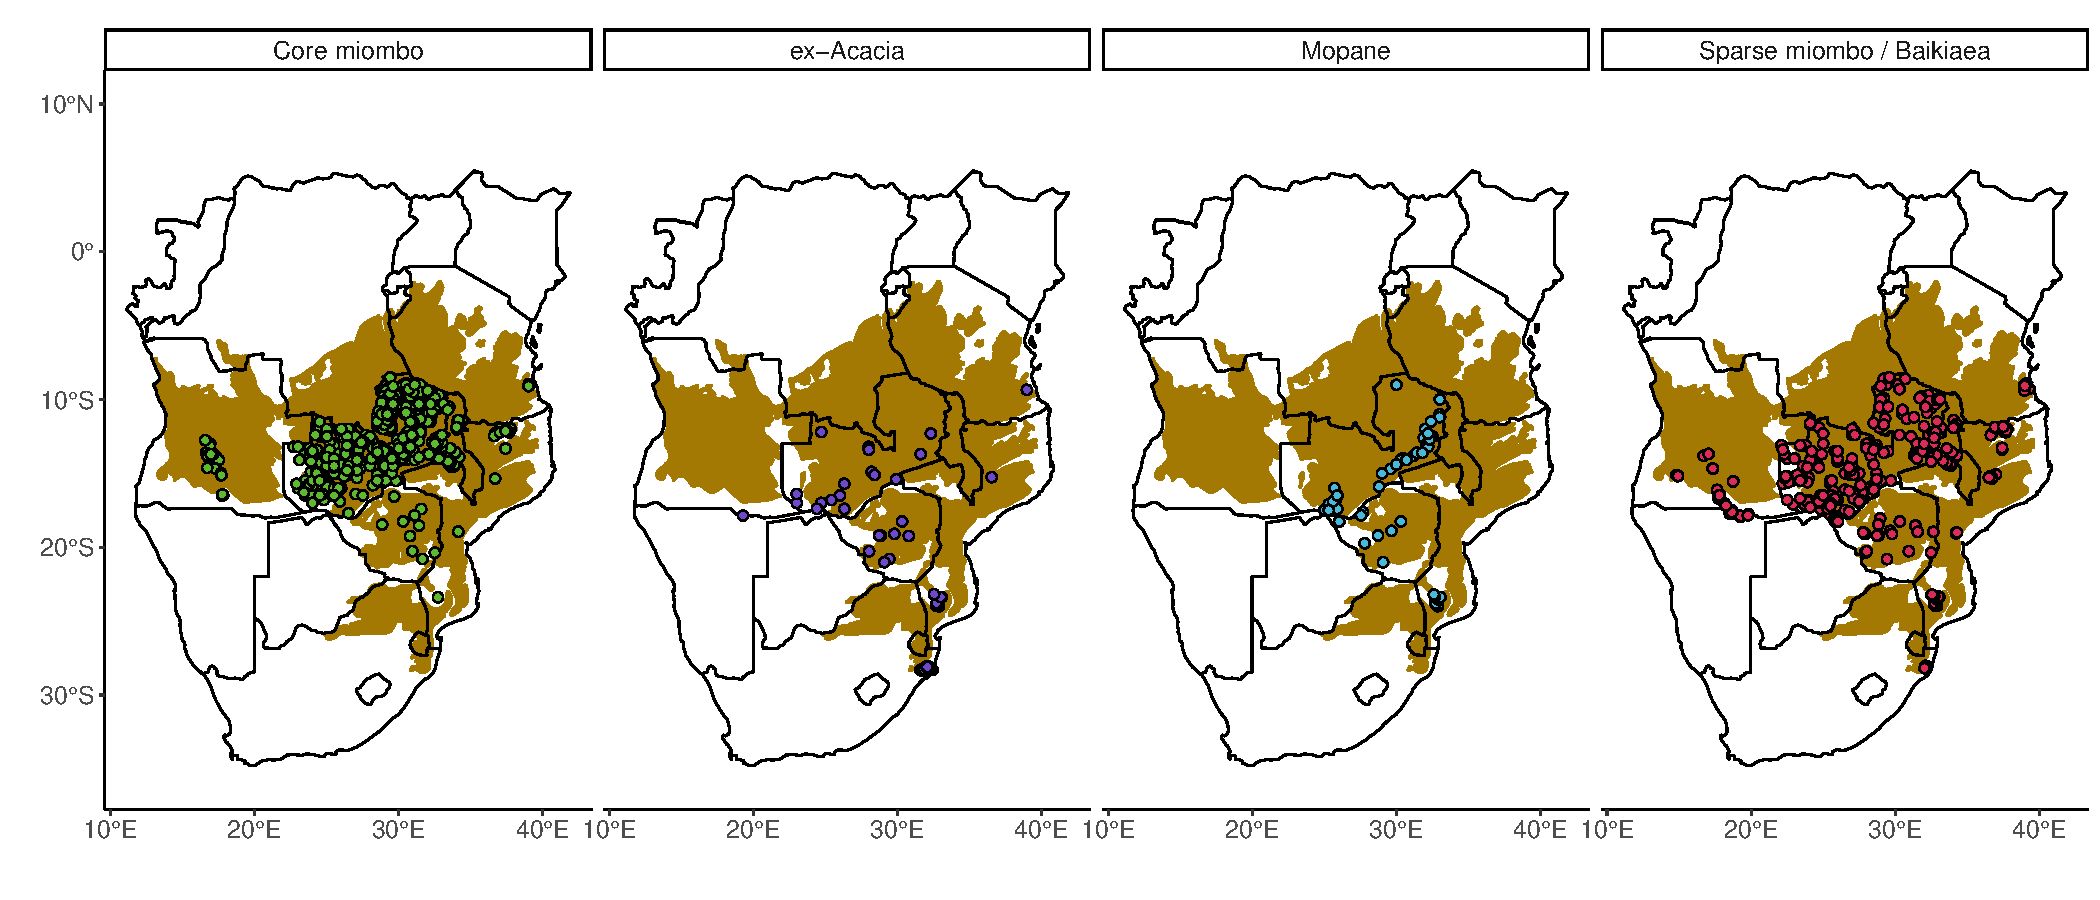
\includegraphics[width=1.4\textwidth]{clust_map}
	\caption{The locations of the \nplots{} plots used in this study, with respect to the distribution of miombo woodland vegetation according to \citet{White1987}. Each panel shows plots categorized by their vegetation type as defined by the vegetation types in \autoref{clust_summ}.}
	\label{clust_map}
\end{figure}
\end{landscape}

\begin{figure}[H]
\centering
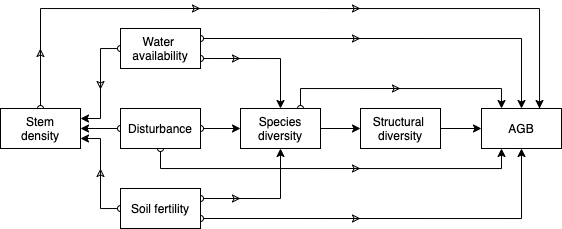
\includegraphics[width=\textwidth]{concept}
	\caption{Conceptual Directed Acyclic Graph (DAG) showing the theoretical relationships between environmental factors, tree species diversity, tree structural diversity, stem density, and AGB. Hypothesised paths of causation are depicted as arrows from predictor to response.}
	\label{con_mod}
\end{figure}

\begin{figure}[H]
\centering
	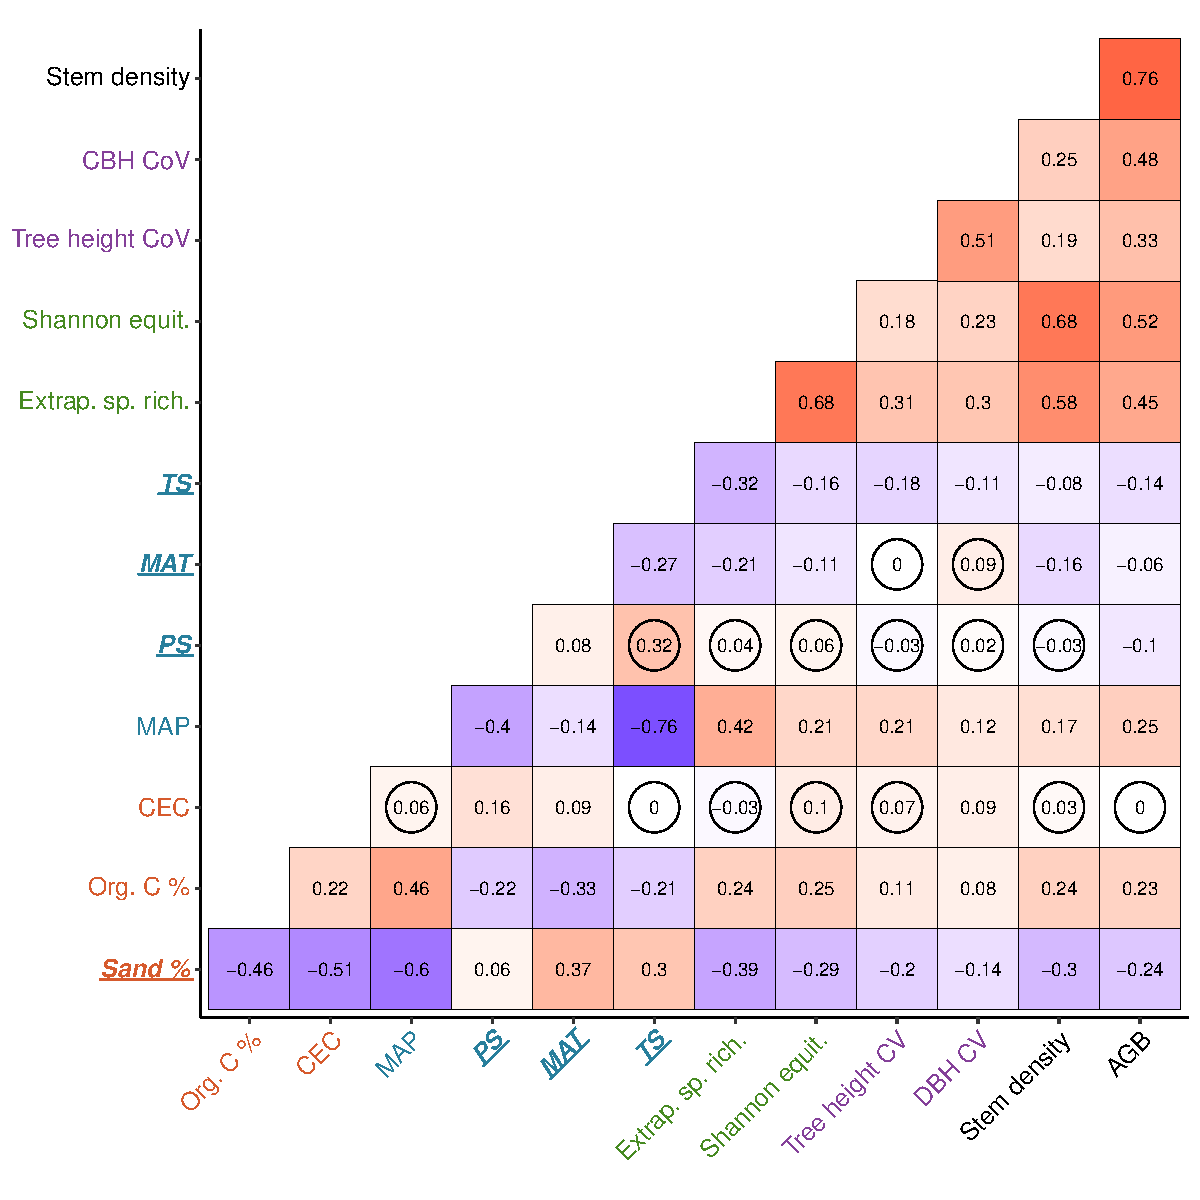
\includegraphics[width=0.6\textwidth]{corr_mat}
	\caption{Correlation matrix of standardised observed variables used in the SEMs, with Pearson correlation coefficients ($r$) coloured according to sign ($+$ve red, $-$ve blue) and shaded by strength of correlation. Correlation coefficients marked by a circle indicate that the 95\% confidence interval of $r$ overlapped zero. Colours of variable names group them into latent variables used in the SEMs: red = soil fertility, blue = disturbance, turquoise = water availability, green = tree species diversity, purple = tree structural diversity. See \hyperref[appendixb]{Appendix B} for a full assessment of correlation fit statistics.}
	\label{corr_mat}
\end{figure}

\begin{figure}[H]
\centering
	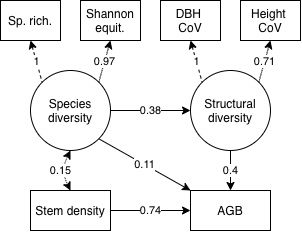
\includegraphics[width=0.5\textwidth]{struc}
	\caption{Path diagram with regression coefficients for the tree diversity SEM, including plots from all vegetation clusters. Latent variables are shown as circles while observed variables are shown as rectangles. Standardised path coefficients are shown as solid arrows pointing from predictor to response with the effect size of the path coefficient expressed in terms of standard deviations on the latent variable response scale. The observed variables that inform the latent variables are connected by dotted arrows, and observed variables with loadings set to one are connected by dashed arrows. Measurement errors of exogenous variables are omitted for clarity.}
	\label{struc_mod}
\end{figure}

\begin{figure}[H]
\centering
	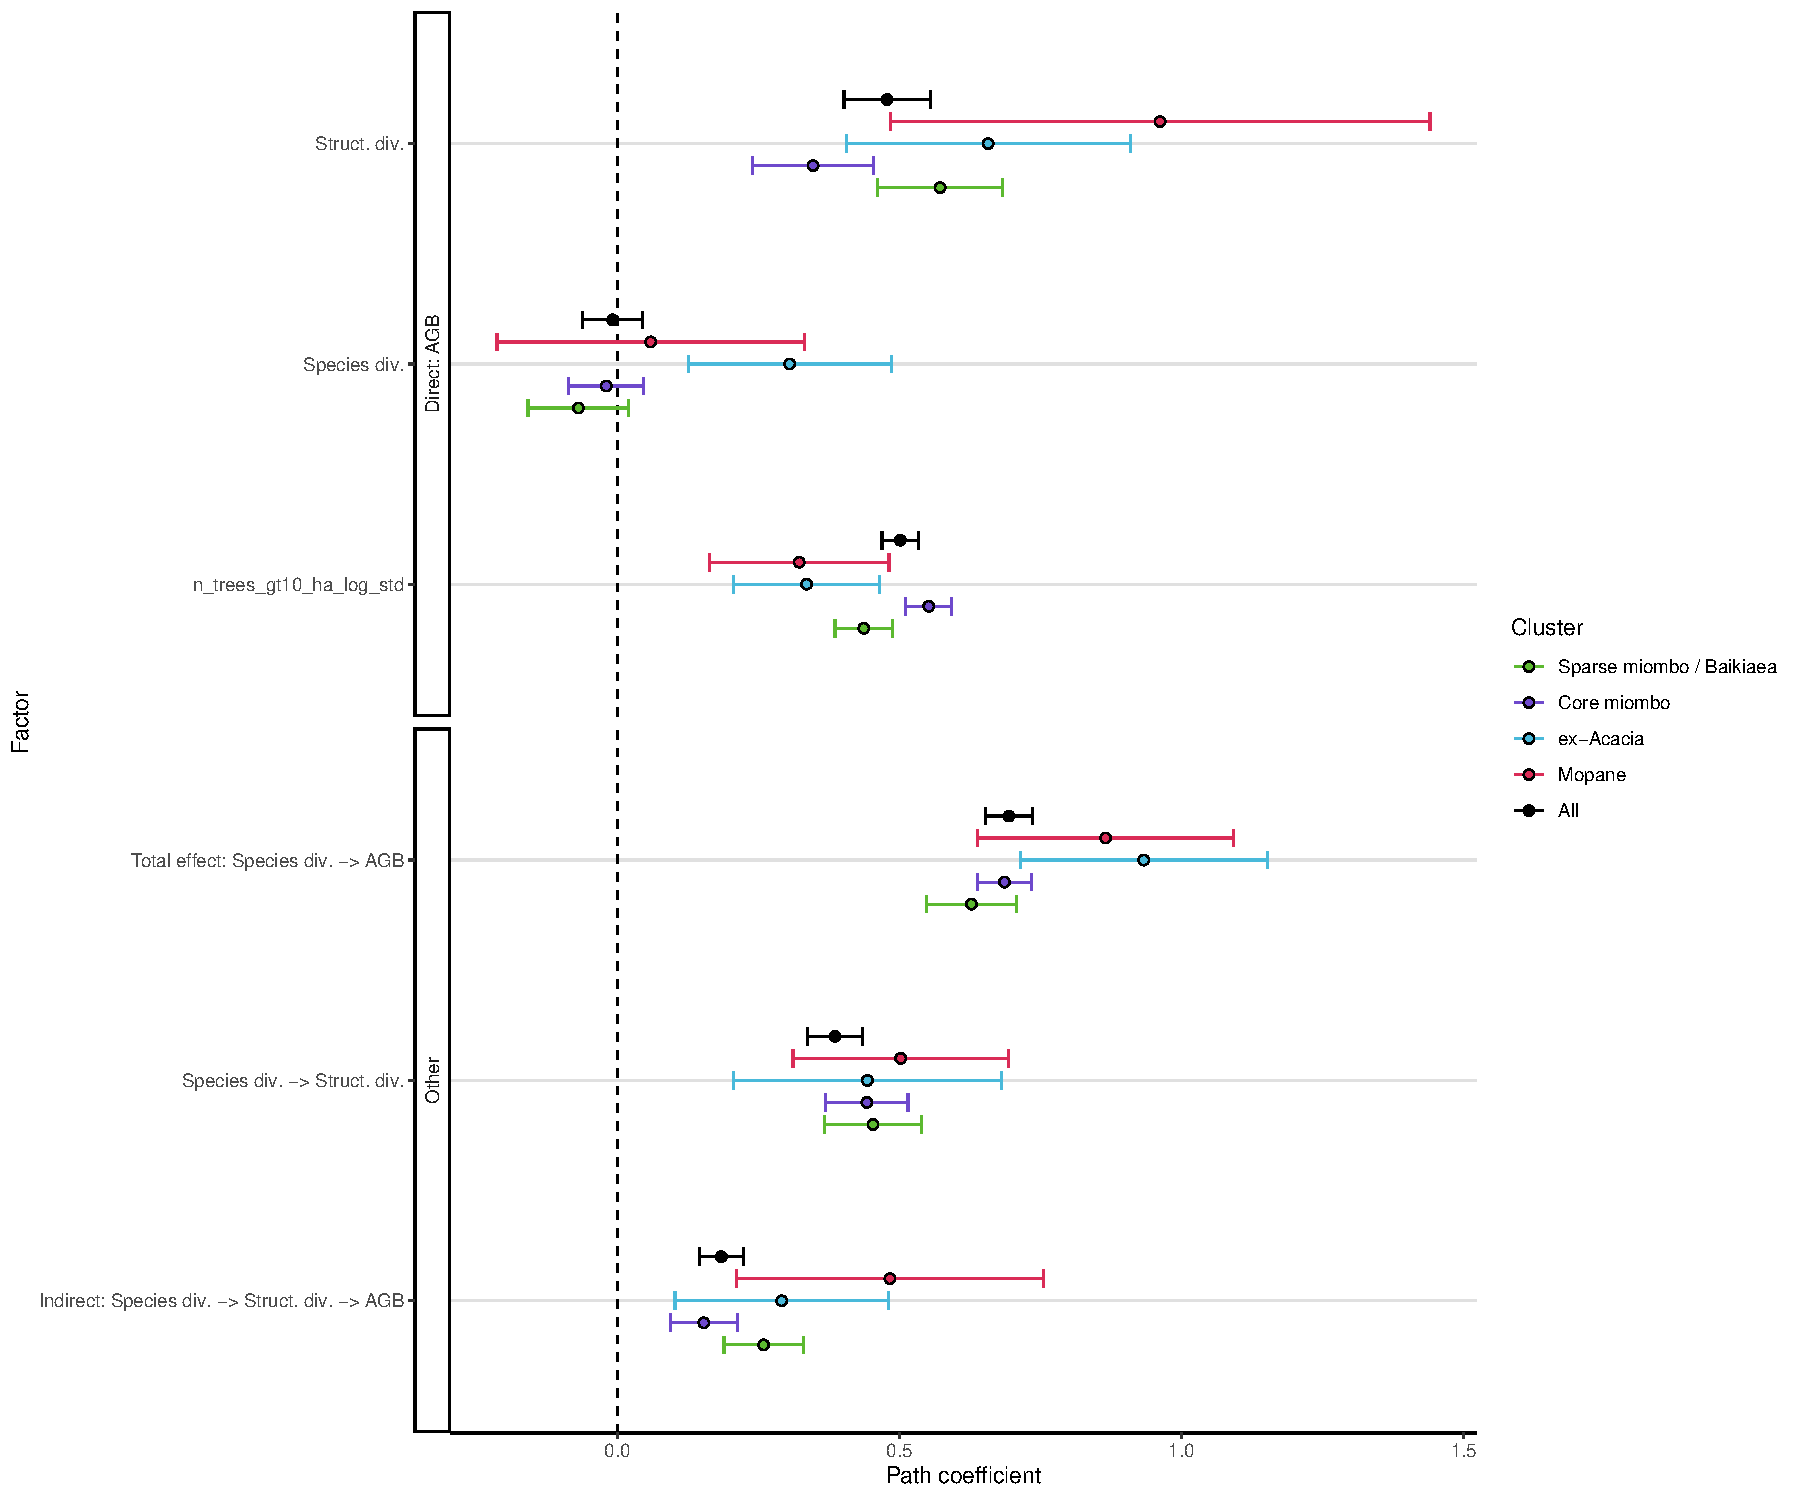
\includegraphics[width=\textwidth]{struc_model_slopes_all}
	\caption{Unstandardised path coefficients for the effects of tree diversity on AGB, mediated by the effect of stand structural diversity. Path coefficients are $\pm$1 standard error. Path coefficients where the interval (standard error) does not overlap zero are considered to be significant effects.}
	\label{struc_model_slopes_all}
\end{figure}

\begin{figure}[H]
\centering
	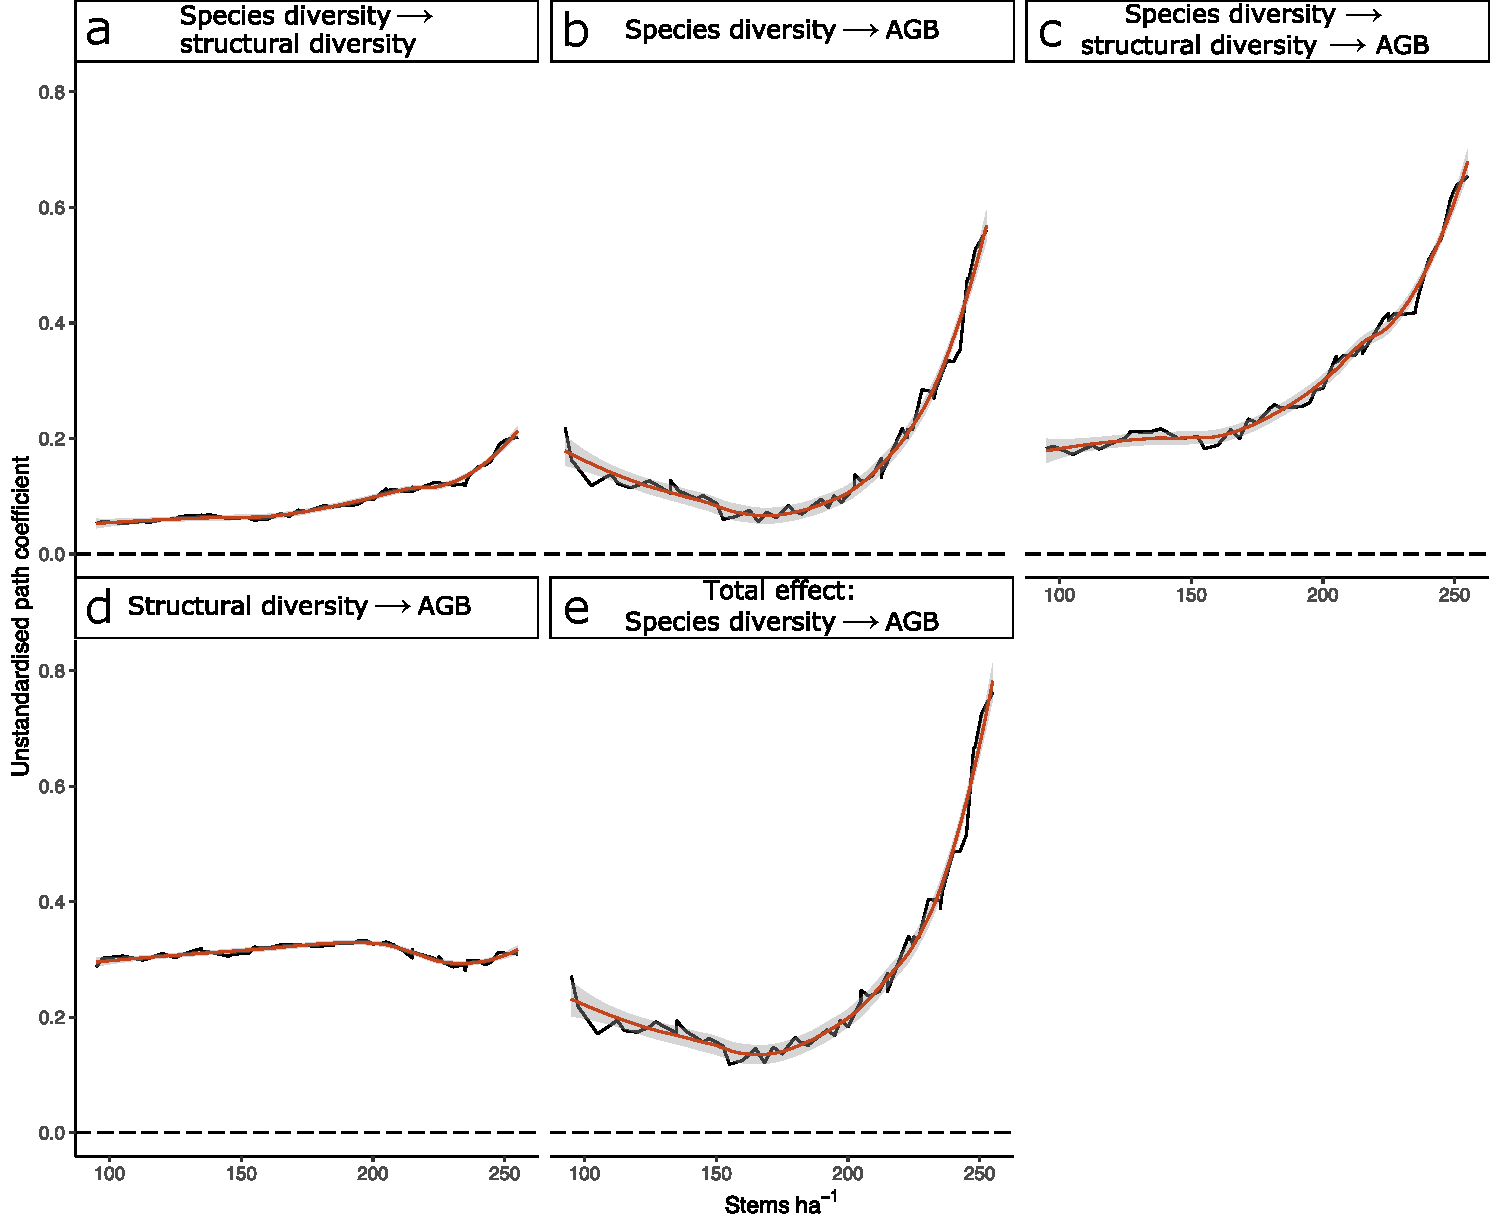
\includegraphics[width=0.8\textwidth]{sem_struc_stems_ha}
	\caption{Line plots showing the variation in path coefficients in the SEM, using datasets with different mean stem density. Smoothed lines are loess curves with standard error shaded bars.}
	\label{sem_struc_stems_ha}
\end{figure}

\begin{figure}[H]
\centering
	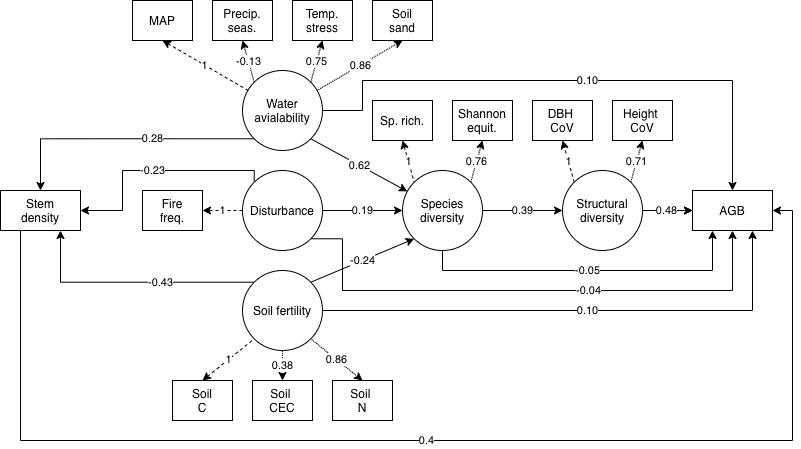
\includegraphics[width=\textwidth]{full}
	\caption{Path diagram with regression coefficients for the SEM incorporating environmental covariates and tree species and structural diversity across all five vegetation types. Latent variables are shown as circles while observed variables are shown as rectangles. Standardised path coefficients are shown as solid arrows pointing from predictor to response, with the effect size of the path coefficient expressed in terms of standard deviations on the latent variable response scale. Observed variables that inform the latent variables are connected by dotted arrows, observed variables with loading set to one are connected by dashed arrows. Measurement errors of exogenous variables are omitted for clarity.}
	\label{full_mod}
\end{figure}

\section{Appendix 1 - Frequency distribution of observed variables} \label{appendixa}

\begin{figure}[H]
\centering
	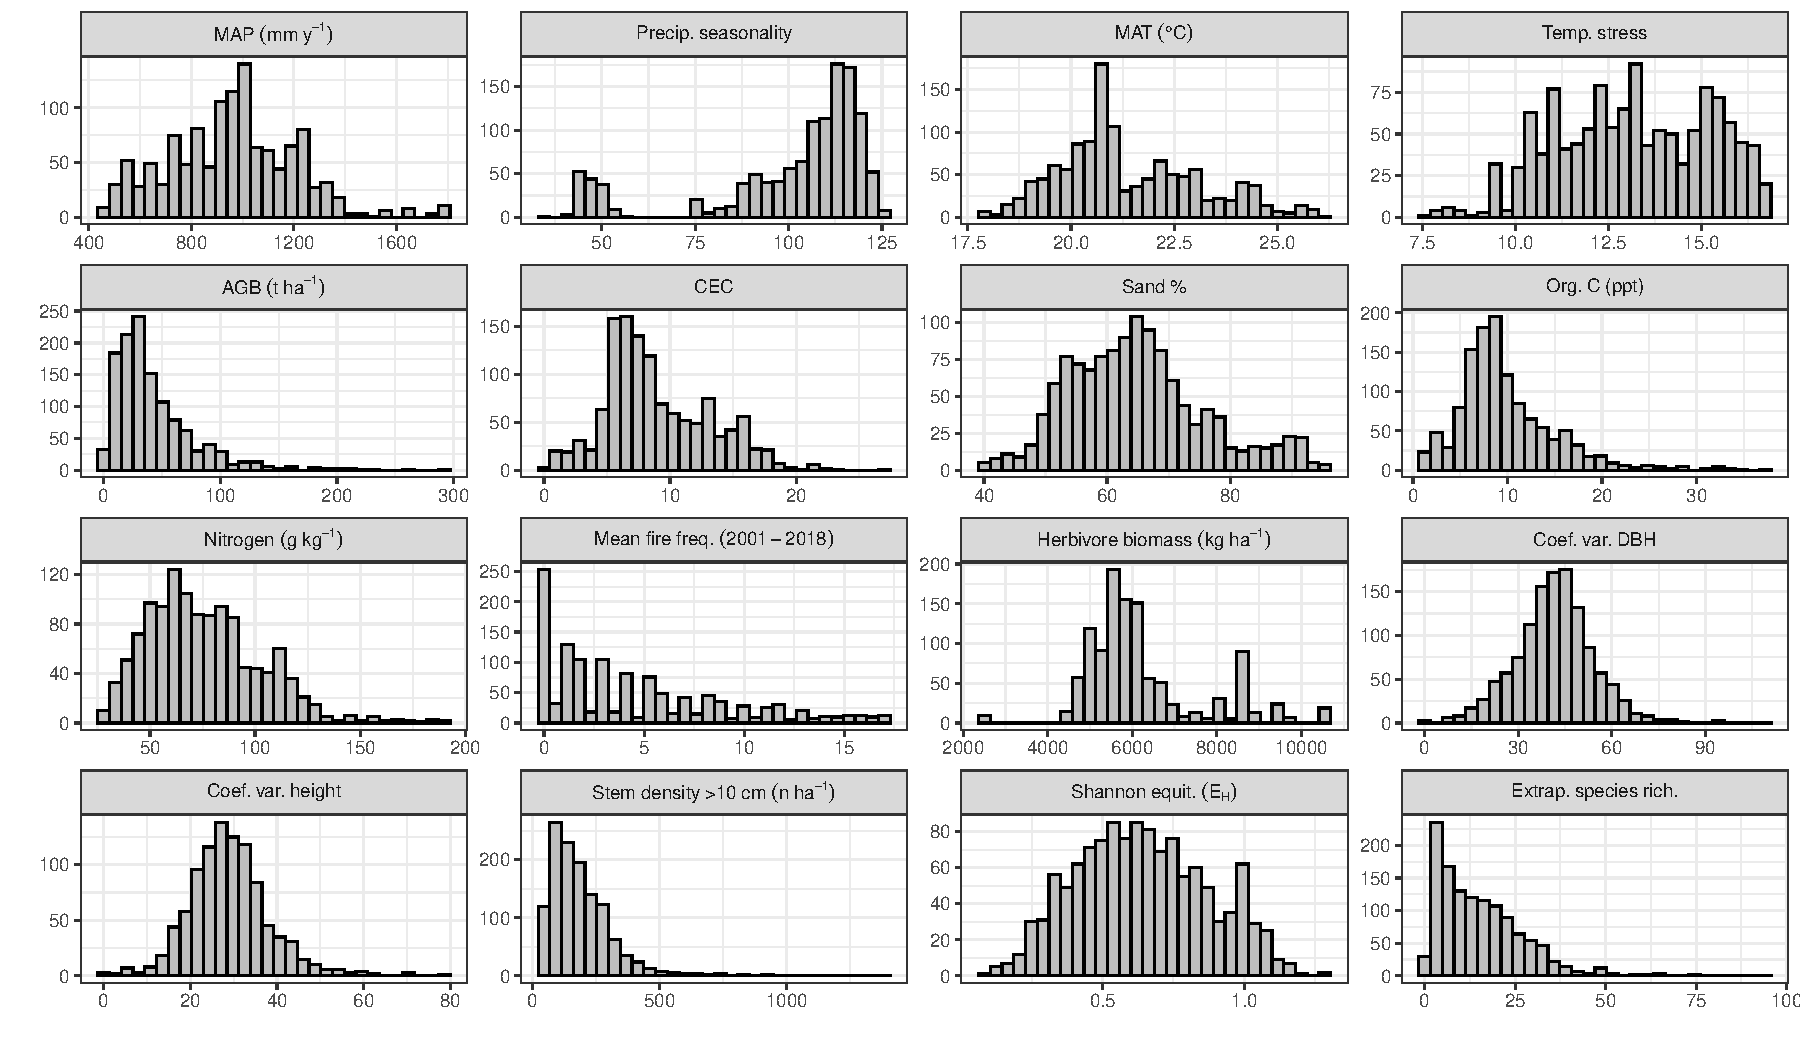
\includegraphics[width=\textwidth]{hist_raw}
	\caption{Histograms of raw untransformed observed variables used in final analyses.}
	\label{hist_raw}
\end{figure}

\begin{figure}[H]
\centering
	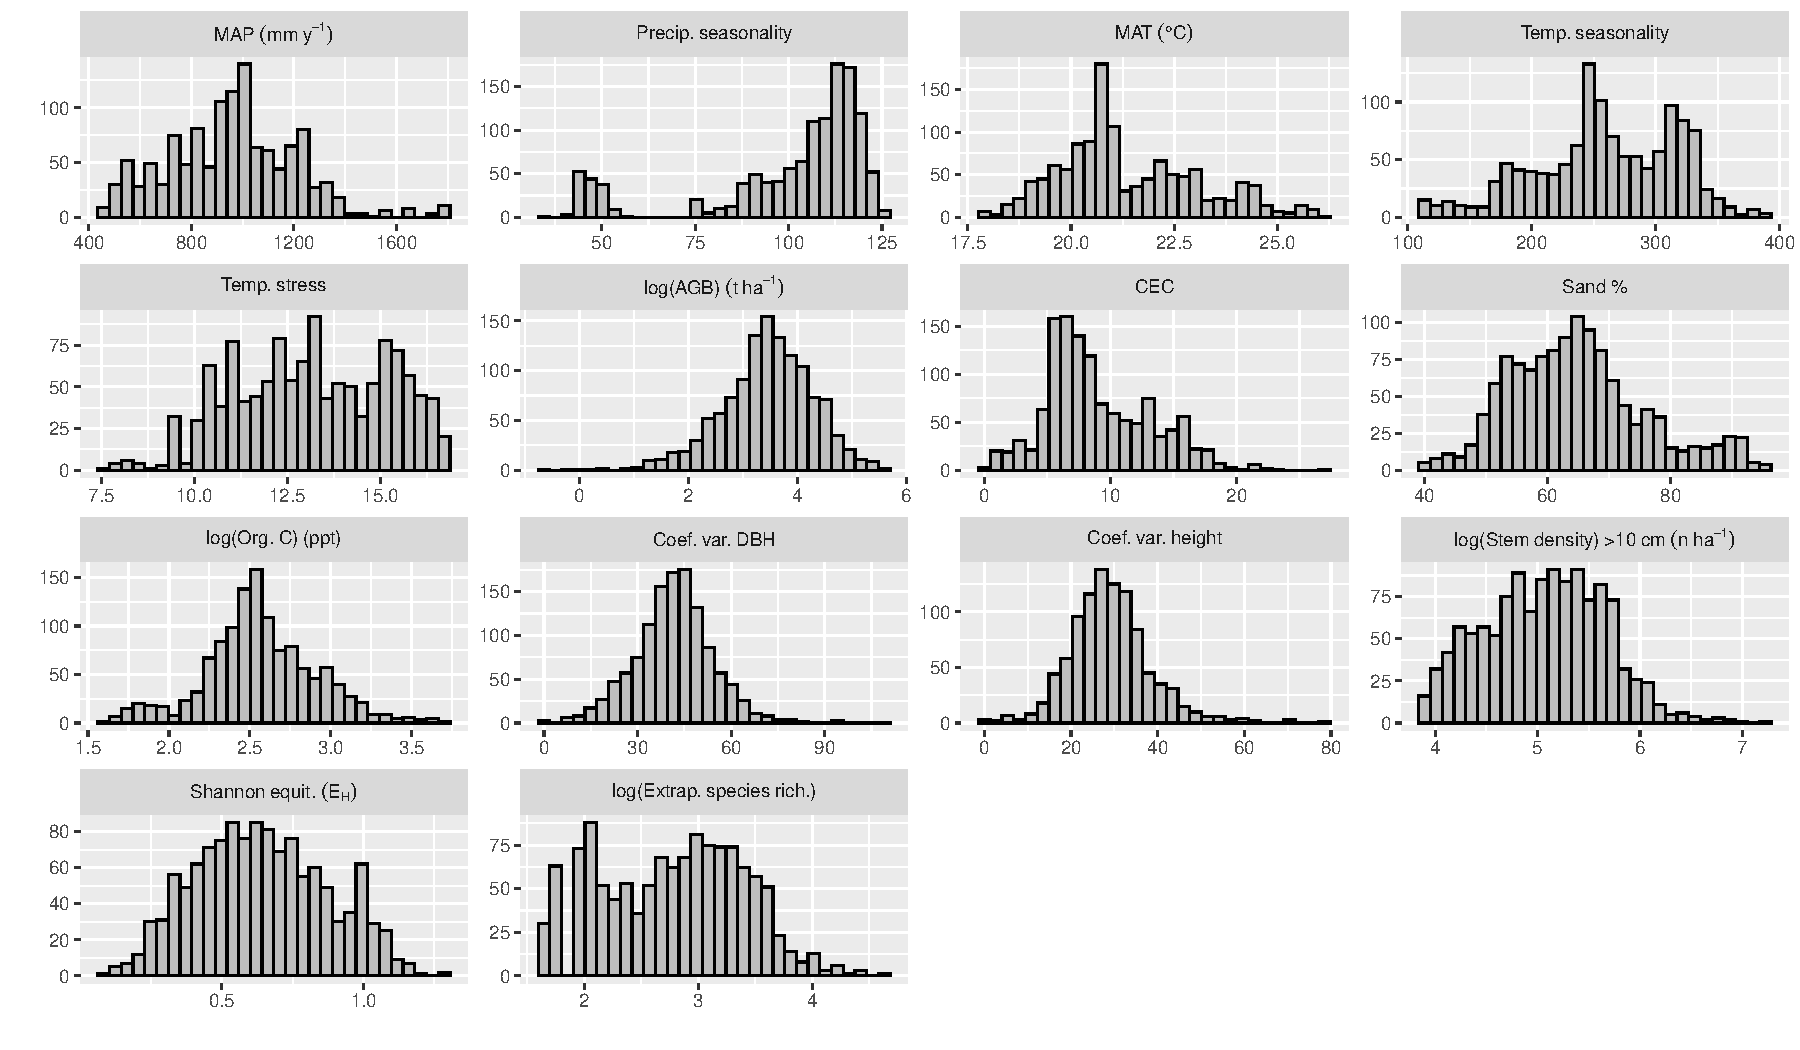
\includegraphics[width=\textwidth]{hist_trans}
	\caption{Histograms of observed variables transformed to achieve a normal frequency distribution.}
	\label{hist_trans}
\end{figure}

\appendix{}
\section{Appendix 2 - Table of correlation fit statistics} \label{appendixb}


% Table created by stargazer v.5.2.2 by Marek Hlavac, Harvard University. E-mail: hlavac at fas.harvard.edu
% Date and time: Wed, Jun 24, 2020 - 13:33:02
\begin{table}[!htbp] \centering 
  \caption{} 
  \label{corr_ci_tab} 
\begin{tabular}{@{\extracolsep{5pt}} ccccccc} 
\\[-1.8ex]\hline 
\hline \\[-1.8ex] 
x\_var & y\_var & raw.r & raw.lower & raw.upper & n & p \\ 
\hline \\[-1.8ex] 
Sand \% & Org. C (ppt) & $$-$0.620$ & $$-$0.650$ & $$-$0.580$ & $1235$ & p \textless 0.01 \\ 
Sand \% & CEC & $$-$0.510$ & $$-$0.550$ & $$-$0.470$ & $1235$ & p \textless 0.01 \\ 
Sand \% & MAP & $$-$0.500$ & $$-$0.540$ & $$-$0.460$ & $1235$ & p \textless 0.01 \\ 
Sand \% & PS & $0.350$ & $0.300$ & $0.400$ & $1235$ & p \textless 0.01 \\ 
Sand \% & MAT & $0.340$ & $0.280$ & $0.380$ & $1235$ & p \textless 0.01 \\ 
Sand \% & TS & $0.380$ & $0.330$ & $0.430$ & $1235$ & p \textless 0.01 \\ 
Sand \% & Sp. rich. & $$-$0.330$ & $$-$0.370$ & $$-$0.280$ & $1235$ & p \textless 0.01 \\ 
Sand \% & Shannon equit. & $0.250$ & $0.190$ & $0.300$ & $1235$ & p \textless 0.01 \\ 
Sand \% & Tree height CV & $$-$0.250$ & $$-$0.300$ & $$-$0.190$ & $981$ & p \textless 0.01 \\ 
Sand \% & DBH CV & $$-$0.170$ & $$-$0.230$ & $$-$0.120$ & $1233$ & p \textless 0.01 \\ 
Sand \% & Stems ha & $$-$0.100$ & $$-$0.160$ & $$-$0.050$ & $1235$ & p \textless 0.01 \\ 
Sand \% & AGB & $$-$0.270$ & $$-$0.320$ & $$-$0.220$ & $1235$ & p \textless 0.01 \\ 
Org. C (ppt) & CEC & $0.460$ & $0.410$ & $0.500$ & $1235$ & p \textless 0.01 \\ 
Org. C (ppt) & MAP & $0.440$ & $0.390$ & $0.480$ & $1235$ & p \textless 0.01 \\ 
Org. C (ppt) & PS & $$-$0.410$ & $$-$0.450$ & $$-$0.360$ & $1235$ & p \textless 0.01 \\ 
Org. C (ppt) & MAT & $$-$0.280$ & $$-$0.330$ & $$-$0.230$ & $1235$ & p \textless 0.01 \\ 
Org. C (ppt) & TS & $$-$0.280$ & $$-$0.330$ & $$-$0.230$ & $1235$ & p \textless 0.01 \\ 
Org. C (ppt) & Sp. rich. & $0.150$ & $0.090$ & $0.200$ & $1235$ & p \textless 0.01 \\ 
Org. C (ppt) & Shannon equit. & $$-$0.160$ & $$-$0.220$ & $$-$0.110$ & $1235$ & p \textless 0.01 \\ 
Org. C (ppt) & Tree height CV & $0.180$ & $0.120$ & $0.240$ & $981$ & p \textless 0.01 \\ 
Org. C (ppt) & DBH CV & $0.140$ & $0.080$ & $0.190$ & $1233$ & p \textless 0.01 \\ 
Org. C (ppt) & Stems ha & $0.090$ & $0.030$ & $0.140$ & $1235$ & p \textless 0.01 \\ 
Org. C (ppt) & AGB & $0.270$ & $0.220$ & $0.320$ & $1235$ & p \textless 0.01 \\ 
CEC & MAP & $$-$0.070$ & $$-$0.130$ & $$-$0.020$ & $1235$ & p \textless 0.01 \\ 
CEC & PS & $$-$0.590$ & $$-$0.630$ & $$-$0.550$ & $1235$ & p \textless 0.01 \\ 
CEC & MAT & $0.170$ & $0.120$ & $0.220$ & $1235$ & p \textless 0.01 \\ 
CEC & TS & $0.070$ & $0.010$ & $0.120$ & $1235$ & p \textless 0.05 \\ 
CEC & Sp. rich. & $$-$0.100$ & $$-$0.160$ & $$-$0.050$ & $1235$ & p \textless 0.01 \\ 
CEC & Shannon equit. & $$-$0.120$ & $$-$0.180$ & $$-$0.070$ & $1235$ & p \textless 0.01 \\ 
CEC & Tree height CV & $0.090$ & $0.020$ & $0.150$ & $981$ & p \textless 0.01 \\ 
CEC & DBH CV & $0.130$ & $0.080$ & $0.190$ & $1233$ & p \textless 0.01 \\ 
CEC & Stems ha & $$-$0.090$ & $$-$0.140$ & $$-$0.030$ & $1235$ & p \textless 0.01 \\ 
CEC & AGB & $0.080$ & $0.030$ & $0.140$ & $1235$ & p \textless 0.01 \\ 
MAP & PS & $$-$0.070$ & $$-$0.130$ & $$-$0.020$ & $1235$ & p \textless 0.05 \\ 
MAP & MAT & $$-$0.200$ & $$-$0.260$ & $$-$0.150$ & $1235$ & p \textless 0.01 \\ 
MAP & TS & $$-$0.770$ & $$-$0.790$ & $$-$0.740$ & $1235$ & p \textless 0.01 \\ 
MAP & Sp. rich. & $0.400$ & $0.350$ & $0.450$ & $1235$ & p \textless 0.01 \\ 
MAP & Shannon equit. & $$-$0.130$ & $$-$0.180$ & $$-$0.070$ & $1235$ & p \textless 0.01 \\ 
MAP & Tree height CV & $0.250$ & $0.190$ & $0.310$ & $981$ & p \textless 0.01 \\ 
MAP & DBH CV & $0.120$ & $0.060$ & $0.170$ & $1233$ & p \textless 0.01 \\ 
MAP & Stems ha & $0.070$ & $0.010$ & $0.120$ & $1235$ & p \textless 0.05 \\ 
MAP & AGB & $0.230$ & $0.180$ & $0.280$ & $1235$ & p \textless 0.01 \\ 
precip\_seas\_std & MAT & $0$ & $$-$0.050$ & $0.060$ & $1235$ & p = 0.95 \\ 
precip\_seas\_std & TS & $0.140$ & $0.080$ & $0.190$ & $1235$ & p \textless 0.01 \\ 
precip\_seas\_std & Sp. rich. & $0.130$ & $0.070$ & $0.180$ & $1235$ & p \textless 0.01 \\ 
precip\_seas\_std & Shannon equit. & $0.070$ & $0.010$ & $0.130$ & $1235$ & p \textless 0.05 \\ 
precip\_seas\_std & Tree height CV & $$-$0.060$ & $$-$0.120$ & $0.010$ & $981$ & p = 0.07 \\ 
precip\_seas\_std & DBH CV & $$-$0.100$ & $$-$0.150$ & $$-$0.040$ & $1233$ & p \textless 0.01 \\ 
precip\_seas\_std & Stems ha & $$-$0.030$ & $$-$0.080$ & $0.030$ & $1235$ & p = 0.33 \\ 
precip\_seas\_std & AGB & $$-$0.190$ & $$-$0.240$ & $$-$0.130$ & $1235$ & p \textless 0.01 \\ 
MAT & TS & $0.060$ & $0$ & $0.120$ & $1235$ & p \textless 0.05 \\ 
MAT & Sp. rich. & $$-$0.170$ & $$-$0.220$ & $$-$0.120$ & $1235$ & p \textless 0.01 \\ 
MAT & Shannon equit. & $0$ & $$-$0.060$ & $0.060$ & $1235$ & p = 0.98 \\ 
MAT & Tree height CV & $$-$0.040$ & $$-$0.100$ & $0.020$ & $981$ & p = 0.2 \\ 
MAT & DBH CV & $0.060$ & $0.010$ & $0.120$ & $1233$ & p \textless 0.05 \\ 
MAT & Stems ha & $$-$0.150$ & $$-$0.210$ & $$-$0.100$ & $1235$ & p \textless 0.01 \\ 
MAT & AGB & $$-$0.090$ & $$-$0.150$ & $$-$0.040$ & $1235$ & p \textless 0.01 \\ 
TS & Sp. rich. & $$-$0.440$ & $$-$0.480$ & $$-$0.390$ & $1235$ & p \textless 0.01 \\ 
TS & Shannon equit. & $0.200$ & $0.150$ & $0.250$ & $1235$ & p \textless 0.01 \\ 
TS & Tree height CV & $$-$0.210$ & $$-$0.270$ & $$-$0.150$ & $981$ & p \textless 0.01 \\ 
TS & DBH CV & $$-$0.090$ & $$-$0.150$ & $$-$0.040$ & $1233$ & p \textless 0.01 \\ 
TS & Stems ha & $$-$0.050$ & $$-$0.110$ & $0.010$ & $1235$ & p = 0.08 \\ 
TS & AGB & $$-$0.180$ & $$-$0.230$ & $$-$0.120$ & $1235$ & p \textless 0.01 \\ 
Sp. rich. & Shannon equit. & $$-$0.580$ & $$-$0.620$ & $$-$0.540$ & $1235$ & p \textless 0.01 \\ 
Sp. rich. & Tree height CV & $0.300$ & $0.250$ & $0.360$ & $981$ & p \textless 0.01 \\ 
Sp. rich. & DBH CV & $0.300$ & $0.250$ & $0.350$ & $1233$ & p \textless 0.01 \\ 
Sp. rich. & Stems ha & $0.240$ & $0.190$ & $0.300$ & $1235$ & p \textless 0.01 \\ 
Sp. rich. & AGB & $0.310$ & $0.260$ & $0.360$ & $1235$ & p \textless 0.01 \\ 
Shannon equit. & Tree height CV & $$-$0.120$ & $$-$0.190$ & $$-$0.060$ & $981$ & p \textless 0.01 \\ 
Shannon equit. & DBH CV & $$-$0.200$ & $$-$0.250$ & $$-$0.140$ & $1233$ & p \textless 0.01 \\ 
Shannon equit. & Stems ha & $$-$0.410$ & $$-$0.460$ & $$-$0.360$ & $1235$ & p \textless 0.01 \\ 
Shannon equit. & AGB & $$-$0.350$ & $$-$0.400$ & $$-$0.300$ & $1235$ & p \textless 0.01 \\ 
Tree height CV & DBH CV & $0.470$ & $0.420$ & $0.520$ & $981$ & p \textless 0.01 \\ 
Tree height CV & Stems ha & $0.010$ & $$-$0.060$ & $0.070$ & $981$ & p = 0.86 \\ 
Tree height CV & AGB & $0.240$ & $0.180$ & $0.290$ & $981$ & p \textless 0.01 \\ 
DBH CV & Stems ha & $0.110$ & $0.060$ & $0.170$ & $1233$ & p \textless 0.01 \\ 
DBH CV & AGB & $0.430$ & $0.390$ & $0.480$ & $1233$ & p \textless 0.01 \\ 
Stems ha & AGB & $0.590$ & $0.550$ & $0.620$ & $1235$ & p \textless 0.01 \\ 
\hline \\[-1.8ex] 
\end{tabular} 
\end{table} 


\section{Appendix 3 - Bivariate relationships of model variables} \label{appendixc}

\begin{figure}[H]
\centering
	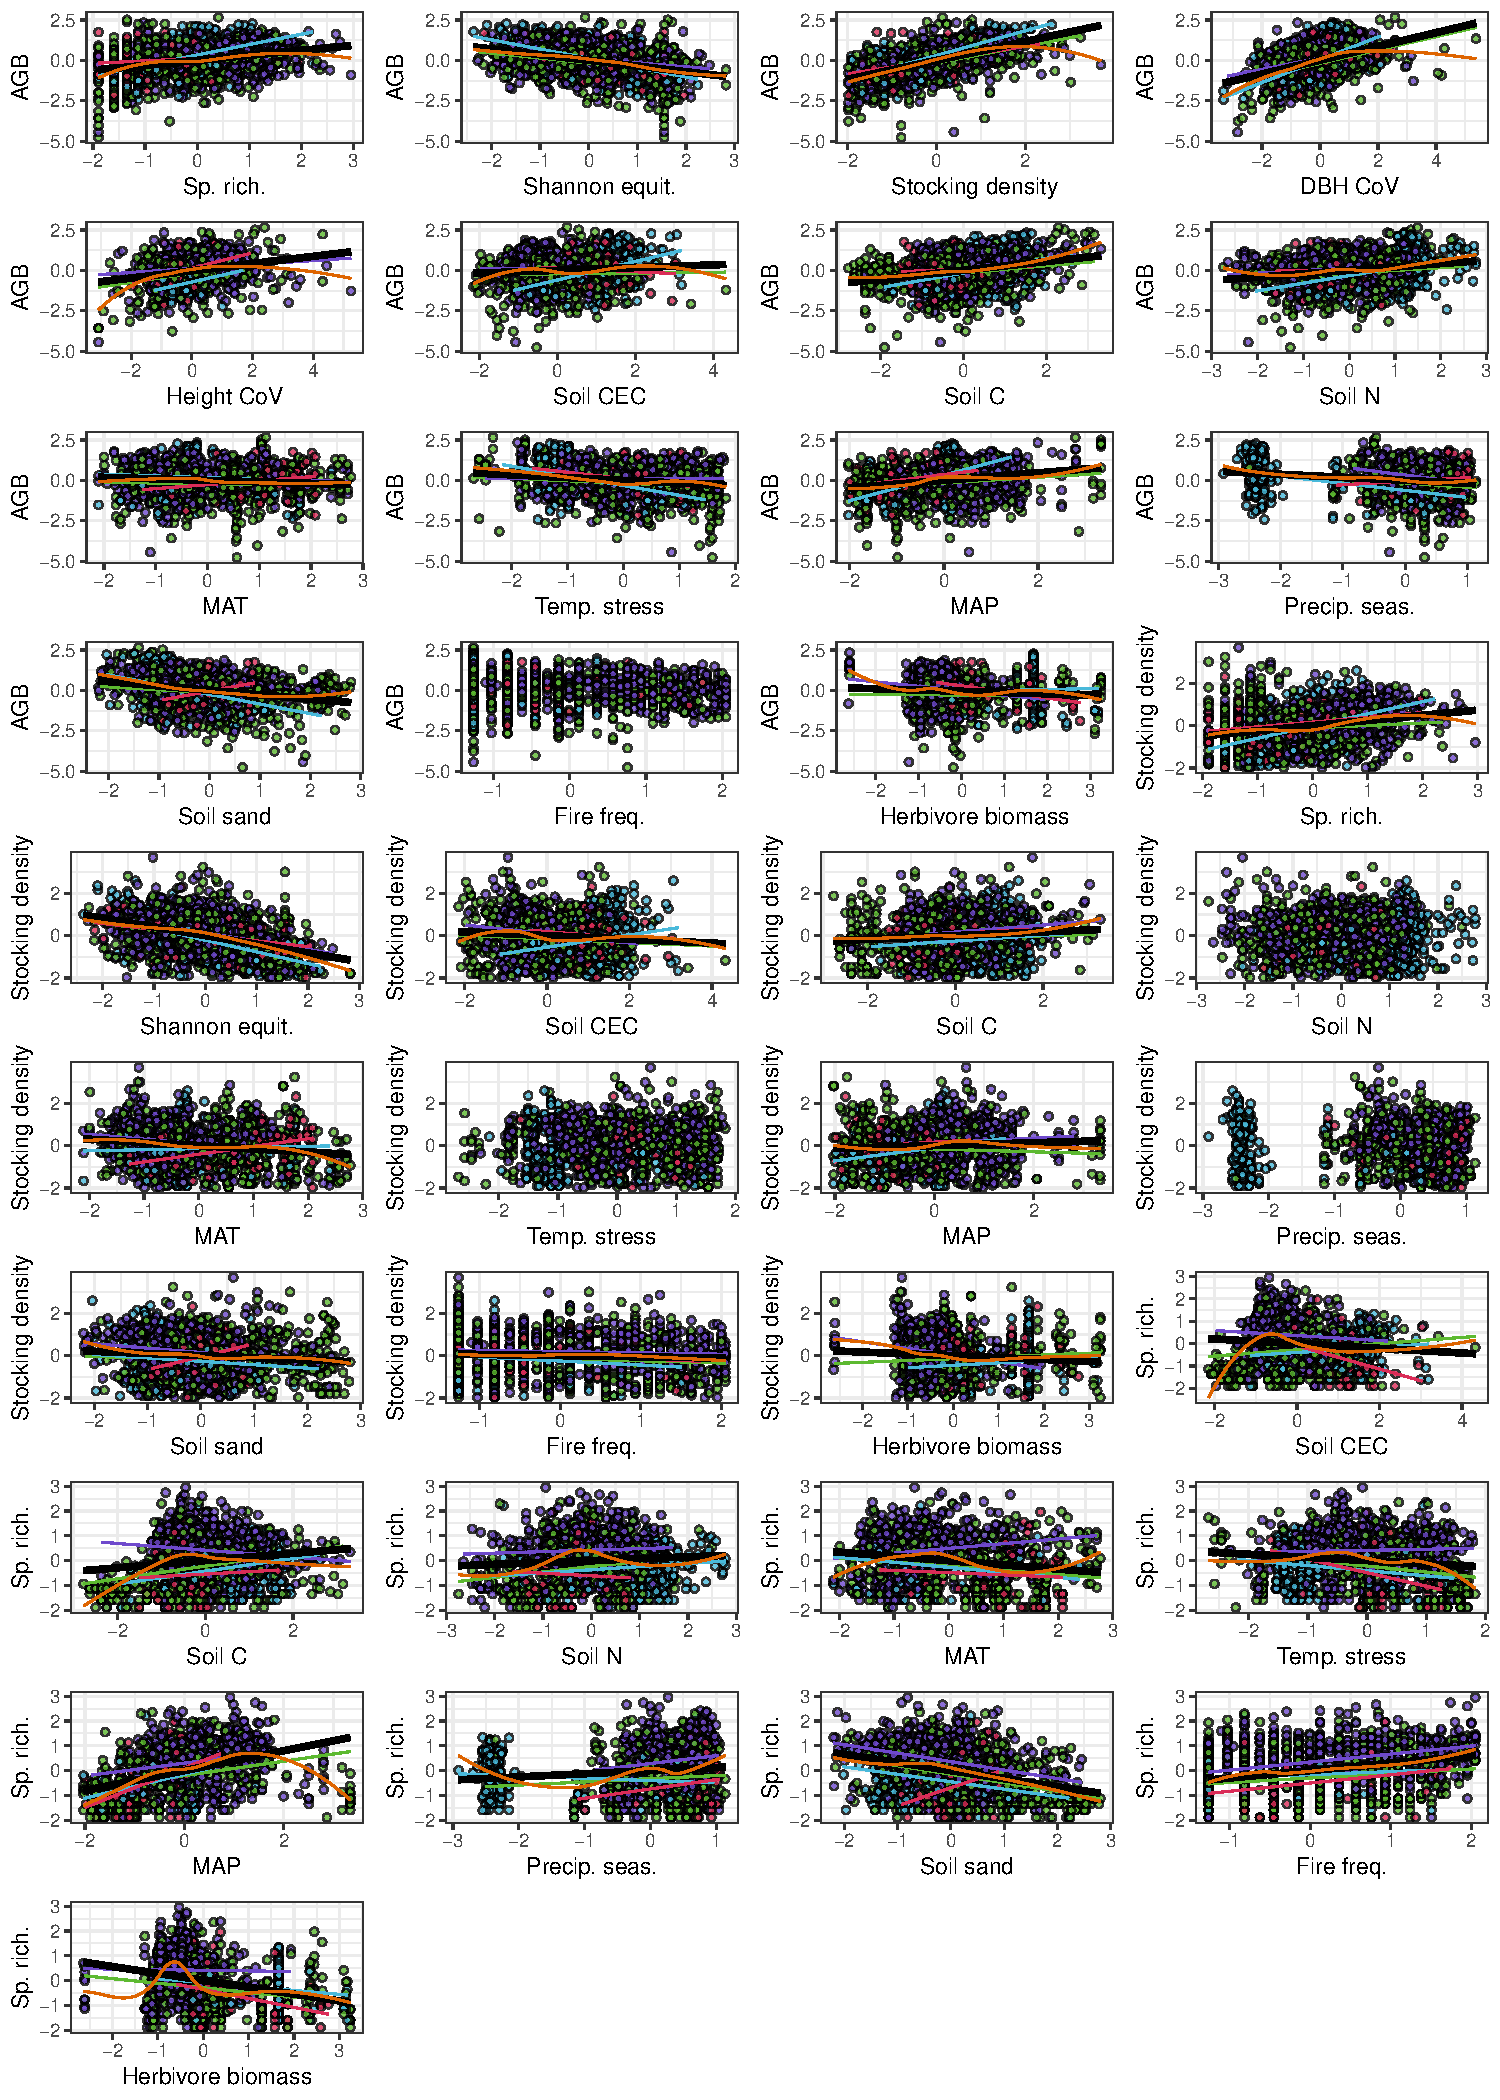
\includegraphics[width=0.9\textwidth]{bivar_lm}
	\caption{Bivariate scatter plots for each observed variable used in the SEMs, based on hypothesised paths of causality. Points are coloured according to vegetation type. A single linear regression is presented as a black line, which combines all vegetation types, separate loess trend lines are fitted for each vegetation type. An orange loess trend line is fitted for all the data. All data is standardised and variables are transformed where it was appropriate for analysis.}
	\label{bivar_lm}
\end{figure}

\section{Appendix 4 - Path coefficients for model incorporating environmental covariates} \label{appendixd}

\begin{figure}[H]
\centering
	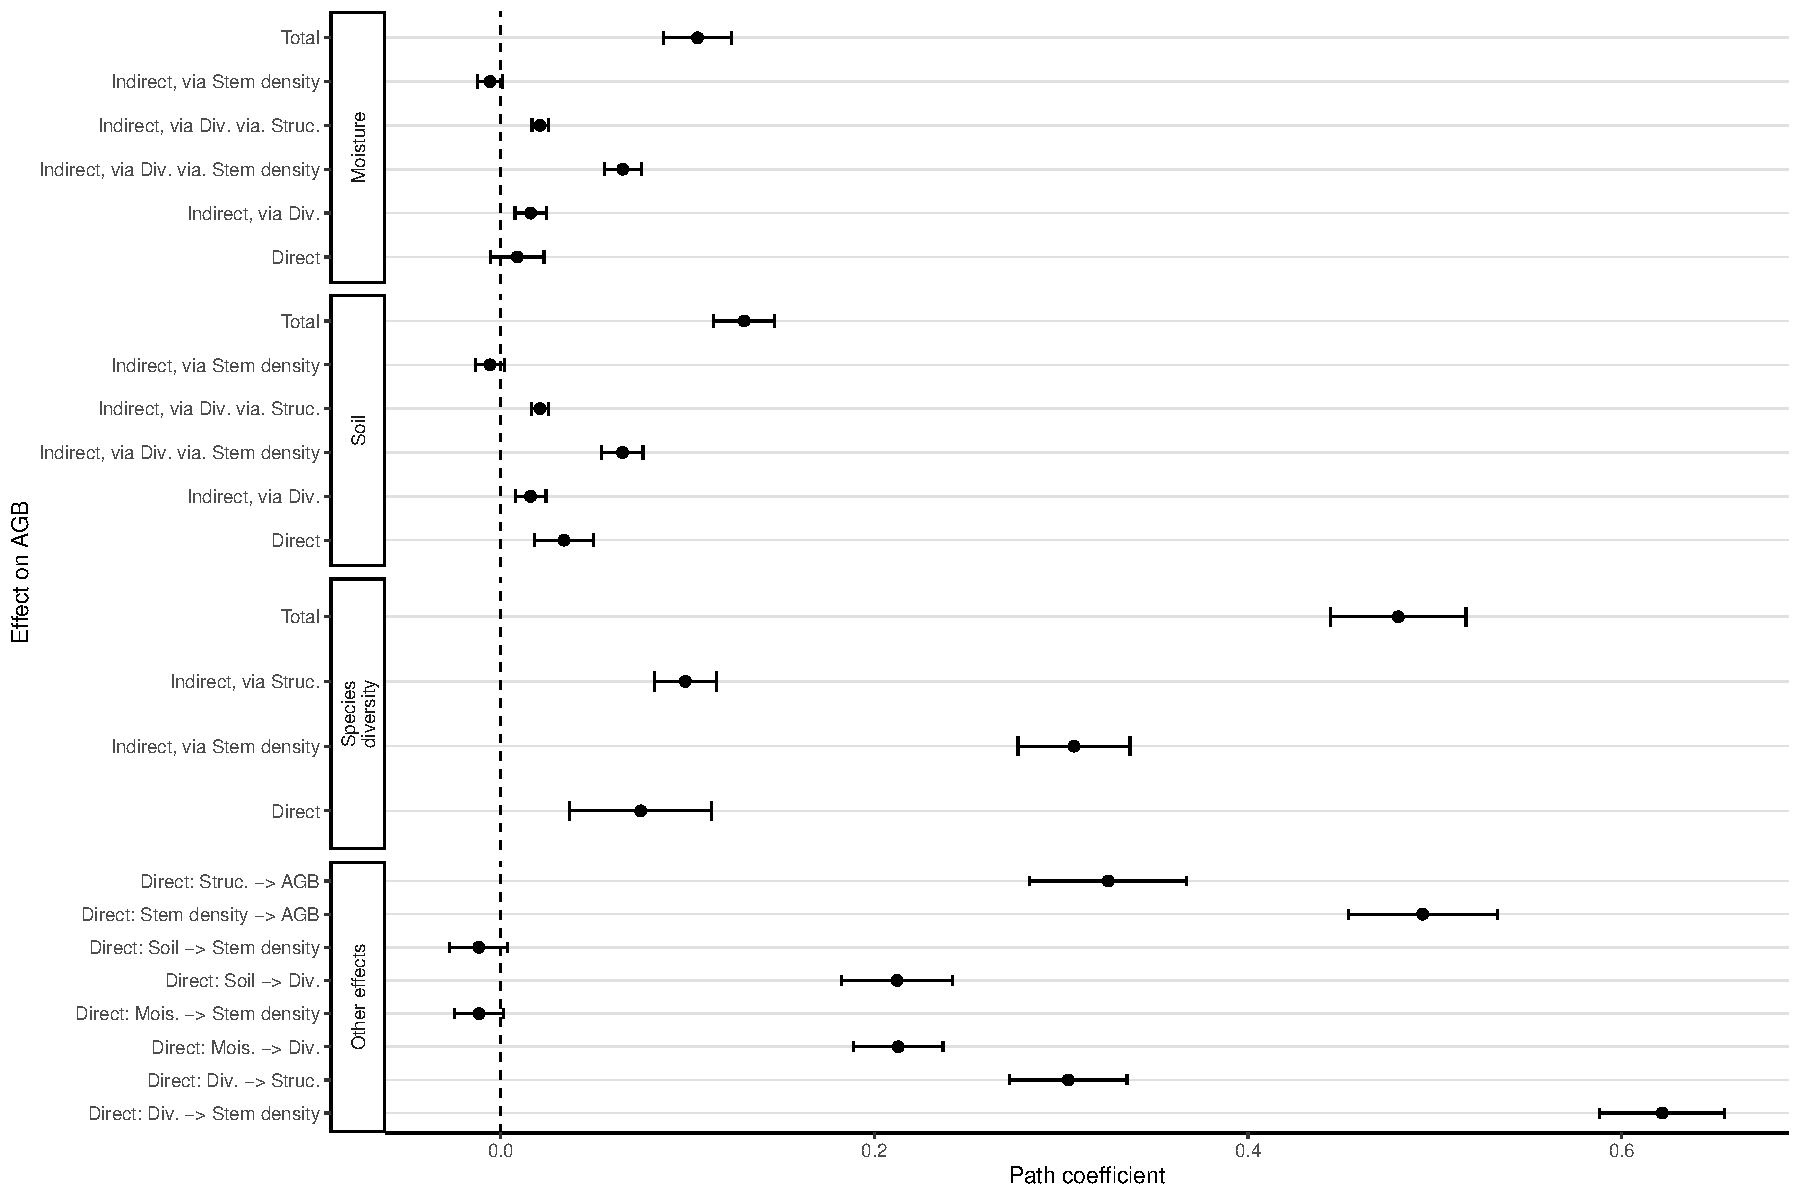
\includegraphics[width=\textwidth]{full_model_slopes}
	\caption{Unstandardised path coefficients for the full model including tree species diversity, environmental covariates and stem density. Path coefficients are $\pm1$ standard error. Path coefficients where the interval (standard error) does not overlap zero are considered to be significant effects.}
	\label{full_model_slopes}
\end{figure}

\end{document}



